\documentclass[print,oneside]{tudelft-report}
% tussen de []-haken van documentclass kun je zetten:
%	[draft] = maakt draft versie: importeert geen plaatjes maar houd daar wel ruimte%	voor, dus compilen gaat veel sneller
%	[print] = maakt print versie: minder gekleurde linkjes
%	[oneside,print] = versie om te lezen op PC, zonder witte pagina's

%% LET OP!
%  aangepast report-class:
%  draft geeft een draft
%  print geeft de juiste versie (andere lettertypes en kleuren enzo)
%%%%%%%%%%%%%%%%%%%%%%%%%%%%%%%%%%%%%%%%%%%%%%%%%%%%%%%%%%%%%%%%%%%%%%%%

% extra packages added
\usepackage[small, bf, hang]{caption} %captions for floats (images etc.)
\usepackage{multicol}
\usepackage{relsize} 		% mathlarger
\usepackage{verbatim}
\usepackage{wrapfig}		% tekst rond figuren
\usepackage[]{placeins}	% gebruik: \FloatBarrier om plaatjes binnen grenzen te forceren
\usepackage{perpage}		% to reset footnotes per page
\usepackage{hyperref}

\usepackage{graphicx}		% voor subfigures
\usepackage{caption}
\usepackage{subcaption}

%\usepackage{tikz}
%\usepackage{pgfplots} 		%voortikz

%%%%%%%%%%%%%%%%%%%%%%%%%%%%%%%%%%%%%%%%%%%%%%%%%%%%%%%%%%%%%%%%%%%%%%%%

% NIEUWE COMMANDO'S
\newcommand{\matlab}{MATLAB}%{\textsc{Matlab}}}
\newcommand{\nexus}{{Google's Nexus 5{\texttrademark} mobile phone}}
\hyphenation{Matlab}
\MakePerPage{footnote}		% to reset footnotes per page

% voor onzichtbare secties Figures
\newcommand\invisiblesection[1]{%
  \refstepcounter{section}%
  \addcontentsline{toc}{section}{#1}%
  \sectionmark{#1}}

%%%%%%%%%%%%%%%%%%%%%%%%%%%%%%%%%%%%%%%%%%%%%%%%%%%%%%%%%%%%%%%%%%%%%%%%
%%%%%%%%%%%%%%%%%%%%%%%%%%%%%%%%%%%%%%%%%%%%%%%%%%%%%%%%%%%%%%%%%%%%%%%%
%%%%%%%%%%%%%%%%%%%%%%%%%%%%%%%%%%%%%%%%%%%%%%%%%%%%%%%%%%%%%%%%%%%%%%%%

\begin{document}

%% Use Roman numerals for the page numbers of the title pages and table of
%% contents.
\frontmatter

\title[]{On Determining Smartphone Microphone Directivity with Application to Beamforming}
\author{R. Brinkman\\T. de Rooij}
\affiliation{Delft University of Technology}
\coverimage{cover/onzecover.jpg}
\makecover

% Titel Samenvatting zo aangepast dat hij netjes onder de inhoudsopgave komt
%\begin{flushright}
%\begin{titlestyle}
%{\Huge\color{toevoeging} Abstract}
%\end{titlestyle}
%\end{flushright}
%% ---------------------------------------
\chapter*{Abstract}
\addcontentsline{toc}{chapter}{Abstract}

An equiangular sampling scheme and accessory measurement set-up for determining the directivity gain pattern of a commercially available smartphone is presented.
Determining this directivity gain pattern based on these measuremenents was not possible, because next to the impulse response of the microphone also the impulse response of the acoustic system.
Different smartphone set-ups are tested and the directivity of a smartphone on a surface differs from a smartphone in mid-air.
The determined directivity gain pattern is suitable for use by a beamforming algorithm, but it resulted in no improvement of the performance of the algorithm.

Interpolation of the measured results was not considered, as the system for which the measurements are intended cannot measure accurate smartphone orientations.
Other work has shown that the orientation of a modern smartphone is not yet known within $10^\circ$ margins, therefore interpolation of the measured results is not considered.
This could be included in future work, along with to the determination of indoor position of a smartphone, a sampling scheme with fewer samples and a means to reverse the contribution of the acoustic system to the measurements.
\chapter*{Acknowledgements}
\setheader{Acknowledgements}
\addcontentsline{toc}{chapter}{Acknowledgements}
\begin{flushright}
Delft, \today
\end{flushright}
For the completion of this project we would like to thank dr. Jorge Mart\`inez-Casta\~neda, our supervisor, without whom we never would have completed this project with these results.
In addition, we would like to thank professor Bastiaan Kleijn, who helped us in the absence of Jorge and gave us some good insights, and dr. Ioan Lager for organizing this years Bachelor graduation project.

We have spend almost two weeks in the anechoic room at the Applied Physics department of the Delft University of Technology to conduct our measurement.
Therefore we would like to thank Henry den Bok, for preparing our measurement set-up, his great tips and always being prepared to help us with little things like connectors which were not at our disposal.

In addition to finishing this thesis, to finish our Bachelor graduation project there were two more parts that had to be completed: the business plan, with special thanks to professor Koen Bertels, and the Ethics course taught by dr. Otto Kroesen.

At last, but not least, we would like to thank our fellow students, with whom we have started and finished this project in a great collaboration: Erik Wouters, Niels van Wijngaarden, Roy Smeding and Sjoerd Bosma.

\begin{flushright}
Rosalie Brinkman \qquad 4111710\\
Tim de Rooij \qquad 4077903\\
\end{flushright}
\cleardoublepage
\addcontentsline{toc}{chapter}{Contents}

\tableofcontents
\setcounter{tocdepth}{2}

\cleardoublepage
\listoffigures

\mainmatter

\chapter{Introduction}
\label{introduction}
\setheader{Introduction}

\begin{figure}[b!]
    \centering
		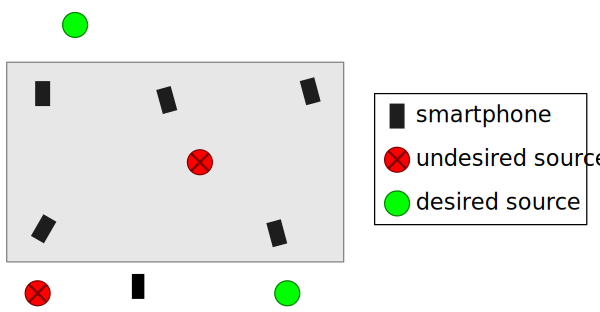
\includegraphics[width=0.6\textwidth]{afbeeldingen/goal_example.png}
	    \caption[Example conference calling system configuration]{An example of a conference calling system configuration}
	    \label{fig:goal}
\end{figure}

A conference call is a telephone call in which two or more parties, possibly consisting of more than one person, can simultaneously communicate.
Conference calls are frequently used in large companies because they allow parties to communicate efficiently without travelling to the same location.
They facilitate team meetings or other occasions in which employees at different locations want to communicate by telephone.

Many large companies currently make use of expensive equipment in specialized rooms.
These systems are often difficult to configure and even then sound quality can not be guaranteed.
Because the audio signals are recorded with one microphone, most of the time positioned at the centre of the table, there is a lot of noise and options for noise cancellation are limited.
A more accessible and convenient solution would be to only use the participants smartphones for such a system: a clear conference call could be held anywhere using a device nearly everyone already possesses.

Another application of such a system could be to help people with hearing aids to communicate.
Someone with a hearing aid has the same kind of problems as a modern conference call system: they cannot filter sounds from different directions, the sound volume is the same from every direction.
For example, when someone with a hearing aid is in a pub, it is very difficult for that person to concentrate on the voices of the people around him.
This is due to the voices of a person at for instance a table to his left being at the same volume as the voice of the person sitting in front of him.
This person could be helped if just a few people placed their smartphones on table and started an application, which connects to the hearing aid and dampens the distracting noises from the other tables at the pub.

An example of a possible conference calling system configuration is shown in Figure \ref{fig:goal}. Several smartphones are located on a table in a regular office environment. A number of desired audio sources (e.g. people speaking) and undesired noise sources (e.g. an air conditioning unit or background conversation) are located around the table. The smartphones are placed in an arbitrary but known positions and the locations of the desired and undesired sources are also assumed to be known. 

The smartphones are running a mobile application from which the sound data is acquired.
This data is then transmitted via a WiFi network and the signals are synchronised in order to make beamforming possible \cite{BAP:RoySjoerd}. 
Beamforming is a technique in the field of signal processing with the purpose to transmit or receive signals directionally \cite{VanVeen19884}.
The described system applies acoustic beamforming.
Hennecke and Fink \cite{hennecke2011towards} concluded that modern smartphones are suitable for acquiring audio signals as input for a beamforming algorithm.
The received signals from the smartphone microphones can be processed into one resulting audio stream.

These microphone signals can be used to amplify the desired signal and suppress background noise.
This is done by spatial filtering, using the given location information of the smartphone microphones and desired and noise sources.
There exist several acoustic beamforming algorithms, each having their own advantages and disadvantages \cite{BAP:ErikNiels}. 
Beamforming will be further explained in this thesis in Section \ref{ssec:background-beamforming}, as this thesis focuses on a three-dimensional directivity gain pattern to improve the result of a beamforming algorithm.
A directivity gain pattern, from now on referred to as \textit{directivity}, gives information about the directional gain of, for instance, a microphone.
The directional gain indicates how a signal of a certain frequency originating from a certain place is attenuated and delayed.

Research on the application of smartphone microphone directivity in a beamforming algorithm has been performed before \cite{Gaubitch2014}, but this research only describes the directivity in one plane and not for all directions.
Still, this research points out that including the two-dimensional microphone directivity in a beamforming algorithm considerably improves the results of the beamforming algorithm. 
It is thus plausible that a three-dimensional microphone directivity will enhance the performance of a beamforming algorithm even more. 
The aim of this thesis is to determine the three-dimensional directivity of a smartphone microphone.
This directivity will be implemented in a larger system to apply beamforming on audio signals recorded by smartphones. 
The directivity behaviour will be determined by examining the impulse response of the microphone for a variety of sample directions.

\begin{figure}[h!]
    \centering
    \includegraphics[width=0.8\textwidth]{afbeeldingen/blokschema4.png}
	\caption[The contribution of the directivity measurements]{The contribution of the directivity measurements in the whole system.}
	\label{fig:system}
\end{figure}

\section{Objective}
An overview of the whole system is shown in Figure \ref{fig:system}.
This thesis describes one of the three parts of the design to make a conference calling system as describe above possible.
The part concerning the smartphone array, including communication between smartphones and the computer, and the synchronisation of the audio signals is left to Bosma and Smeding \cite{BAP:RoySjoerd}.
The implementation of different beamforming algorithms and the quality comparison for these different algorithms was performed by Van Wijngaarden and Wouters \cite{BAP:ErikNiels}.

The green box marks the study of this thesis: determining the directivity gain pattern of a smartphone microphone and apply this directivity to a beamforming algorithm.
This thesis will describe the process of measurement, processing and displaying the data.
An important question that needs to be answered is how representative one measurement is for different settings of the smartphone and for different phones of the same type. 
For this project \nexus~ is used. Not much information is available about the microphones used in this smartphone or their directivities.
Therefore the directivities of the microphones will have to be determined by measurement, with as much accuracy as possible in the given time. 
The objectives for the function, as a part of the beamforming system, are specified more precisely in the schedule of requirements, in Appendix \ref{app:requirements}. 

%\FloatBarrier
\section{Thesis structure}
This thesis starts with the theoretical background of measuring microphone directivities in Chapter \ref{chap:background}.
Subsequently the available resources, measurement set-up and decisions made will be discussed in Chapter \ref{chap:measurements}.
The results of these measurements were not directly usable, but needed to be equalized to support the beamforming algorithm.
This process is described in Chapter \ref{chap:equalization}.
After this, the final results and a discussion of these results will be presented in Chapter \ref{chap:outcome} in Section \ref{sec:results} and Section \ref{sec:discussion} respectively.
Finally, a conclusion and our recommendations for future work are presented in \ref{chap:conclusion}. \\
Ethical considerations regarding the project are added in Appendix \ref{app:ethical}.

\section{Definitions and notation}
Throughout this thesis, there will be definitions and (mathematical) notation, which will be presented in advance.
If $x[n]$ is a discrete time signal, with N entries and $n=1,2,\ldots,N$, $\mathbf{x}$ is the vector notation of the signal and $X[\omega]$ ($\mathbf{X}$ in vector) is its discrete Fourier domain counterpart.
$\mathbb{N}_0$ denotes the set of natural numbers, with 0 includes: 0, 1, 2, 3,$\ldots$ and $\mathbb{N}$ denotes the set of natural numbers larger than 0: 1, 2, 3, 4,$\ldots$.
For matrices non-bold capitals will be used.
The convolution $c[n]$ of two signals $a[n]$ and $b[n]$ is written using an asterisk:
\begin{equation*}
c[n]=(a*b)[n].
\end{equation*}

For vector multiplication, assume two vectors $\mathbf{a}$ and $\mathbf{b}$, then its dot product or inner product $\mathbf{c}$ is written as:
\begin{equation*}
\mathbf{c}=\langle \mathbf{a},\mathbf{b}\rangle
\end{equation*}
and its cross product or vector product $\mathbf{d}$ written as:
\begin{equation*}
\mathbf{d}=\mathbf{a}\times\mathbf{b}.
\end{equation*}

For rounding the following signs are used:
$\lceil\bullet\rceil$
for rounding up and
$\lfloor\bullet\rfloor$
for rounding down.

Quantities in this thesis are often expressed on a logarithmic scale using decibel (dB) units.
Since the units in these thesis are field units (unless specified otherwise), the field unit form of the decibel scale is used:
\begin{equation*}
20\log_{10}|\bullet|.
\end{equation*}
From this follows the inverse of the dB-scale:
\begin{equation*}
10^{\dfrac{\bullet}{20}}.
\end{equation*}

The definitions of the spherical coordinate-system can be found in Figure \ref{fig:bol_def}.
The azimuth, $\theta$, is the angle between the projection of the vector pointing from the origin to the point on the $x,y$-plane and the $x$-axis.
The elevation, $\phi$, is the angle between the projection of the vector pointing from the origin to the point on the $x,z$-plane and the $z$-axis.
In Figure \ref{fig:def_nexus}, the definitions of the different sides of a smartphone are given.
The top of the smartphone, we will be called the listeningside, the bottom the speechside, the left side of the screen is the left side of the phone, the other side is the right side.
For specifying the orientation of the phone, the terms `screen up' and `screen down'  or `face up' and `face down' are also used.

If the phone is placed in the spherical coordinate system, the listeningside of the phone is pointing towards $(\phi,\theta)=(90^\circ,0^\circ)$.
Laying in the $(x,y)$-plane, with the screen face up towards the $+z$-direction.

The last thing to note is that all code for this thesis was written for \matlab~ Student R2014a. For some some of the hardware used in this thesis special drivers are needed, which can be found via the reference given when the hardware is mentioned.

\vspace{1in}

\begin{figure}[h]
\centering
\begin{subfigure}[t]{0.45\textwidth}
    \centering
    \includegraphics[width=\textwidth]{afbeeldingen/azel.jpeg}
    \caption{Definitions on a sphere, azimuth $\theta$, elevation $\phi$}
    \label{fig:bol_def}
\end{subfigure}~
\begin{subfigure}[t]{0.45\textwidth}
    \centering
    \includegraphics[width=\textwidth]{afbeeldingen/nexus_sides.jpg}
    \caption{Definitions of the different sides of the smartphone. Picture of {\nexus} used from \cite{nexus:figure}.}
    \label{fig:def_nexus}
\end{subfigure}
\caption[Definitions in this thesis]{Definitions used throughout this thesis.}
\label{fig:def}
\end{figure}
\chapter{Background}
\label{chap:background}
\setheader{Background}

In this chapter most of the theory about measuring the directivity of a smartphone microphone is addressed.
The related research will be discussed first, after which the operations of a beamforming algorithm is briefly explained, followed by a comparison between different sampling schemes for spherical sampling and methods to measure the impulse response.
Of these impulse response determination methods, two techniques will be explained in more detail, since they will be used in the measurements (further explanation of this choice is given in Chapter \ref{chap:measurements}).
In the next chapter, the final choices concerning the directivity measurements  will be made on base of this presented theory.   

\section{Related Research}
This research is a continuation of the work of Gaubitch et al. \cite{Gaubitch2014}, who concluded the directivity of a smartphone microphone could be used to improve beamforming algorithms.
While some smartphone directivity measurements were already conducted for this paper, these were only performed in a two-dimensional plane around the smartphone, instead of a full three-dimensional sphere \cite{Gaubitch2014}.
The smartphone available for the measurements is \nexus~ \cite{nexus5}.
No information about the microphone used in this mobile phone is made available by Google \cite{nexus5} or LG \cite{nexus5:lg}, the two parties that produced it.
Information about microphone control and automatic gain control from the smartphone is also not given \cite{BAP:RoySjoerd}.

Determining the directivity is, in short, determining the impulse response of the microphone with respect to signals from different directions.
This comes down to two parts: impulse response determination and sampling in space.
To take the measured directivities into account in the beamforming algorithm, the measured results must be converted to a more suitable form for the algorithm.
The directivities are measured for a certain number of data points. The beamforming algorithm also needs the directivities for an intermediate value, thus interpolation is necessary. 
These interpolation calculations will take time and computing power, a possible source of trouble in the beamforming algorithm \cite{BAP:ErikNiels}. 
The algorithm will use the information from the measurements multiple times per second \cite{BAP:ErikNiels}, so performing this interpolation during the actual beamforming is undesirable. Instead, all the interpolation is done as a preprocessing step as the algorithm only works with non-moving and known places in space \cite{BAP:ErikNiels}. As a result, when directivity data for a given orientation is requested, only a look-up is performed

In the next section, the operations of a beamforming algorithm is discussed, as well as how to account for the directivity of (for instance) a smartphone microphone in these algorithms.

\subsection{Beamforming}
\label{ssec:background-beamforming}
This thesis is about the directivity of a smartphone microphone, which is to be used in a beamforming algorithm.
It is therefore important to know more about beamforming in general, to specify the type of beamforming used in this research and to recognize the role of the microphone directivity in such an algorithm.  


Beamforming is a widely used technique in the field of signal processing with the purpose to transmit or receive signals directionally.
Several algorithms for achieving this goal are described in the literature \cite{mucci1984comparison}.
Beamforming makes use of an array of sensors to achieve spatial filtering \cite{VanVeen19884}.
A beamformer processes the spatial samples of propagating wave fields, collected by the sensor array.
Signals with overlapping frequency content but different spatial origin are separated.
Desired signals from a certain direction can then be estimated despite the presence of noise and interfering signals. 
In this way, the beamformer can select the desired signal and eliminate the undesired one. 

Because of the variety of beamforming applications, several distinctions have to be made to determine the type of beamforming in this project.
The beamforming discussed here is about voice signal reception with smartphone microphones.
Beamforming can be used with different types of sensor arrays. Sensor arrays may vary in geometry, number and size \cite{VanVeen19884}.
The array geometry could vary from linear, circular, spherical to arbitrary geometries.
This research focuses on so-called ad-hoc microphone arrays, which are microphone sensor arrays with arbitrary geometries \cite{BAP:ErikNiels}. 

Beamforming can be classified as either near-field or far-field, with different algorithms required for each. The situation depends on the dimensions of the array \cite{ryan1997near}.
If the wave field originates from a distance far greater than the dimensions of the array, the situation can be considered far-field.
There will be no difference in Direction of Arrival (DOA) for every sensor in the array, because the wave field can then be assumed to have a flat wave front.
However, in the case of near-field beamforming the distance between the source and the array is comparable to the dimensions of the array.
This will lead to a noticeable difference in DOA and amplitude of the signal at every sensor.  
During a conference call, the distance between the participant (source) and the smartphone microphone will be small. Therefore, this is considered a near-field scenario \cite{BAP:ErikNiels}. 

The last distinction to be made concerns the choice between broadband and narrowband beamforming techniques \cite{brandstein2001}. This choice depends on the signals incident on the array. The size of an array in terms of operating wavelength is important in measuring array performance. Consider a linear array with a fixed number of elements and fixed inter-element distance. For high frequency signals (with small wavelength) incident on the array, this fixed array will appear large and the main beam will be narrow. In case of low frequency signals (with large wavelength), this same array will appear small and the main beam appears wide. 
For application of the processed signals in speech communication the beamforming algorithm has to operate well in a frequency band from 300 Hz to 3500 Hz \cite{doclo2003design}.
A speech signal is a very wideband signal, which covers some four octaves. If a speech signal is used in a narrowband array, this will give a disturbing speech output. This is the result of a varying beam width caused by the wide frequency range. The interfering signal will not be uniformly attenuated but instead low-pass filtered over its entire band \cite{brandstein2001}. 
In speech applications the narrowband assumption is therefore never valid and a beamformer designed specifically for broadband applications need to be used. 

Beamforming with smartphone microphone arrays is a form of acoustic beamforming. It can be applied in a room with multiple speakers, which is the case during a conference call.
The desired signal originates from a speaker's mouth and is hindered by the signals caused by other speakers and room reverberation \cite{brandstein2001}.
In this case, spatial filtering can be applied because the interfering sources usually originate from points in space apart from the unwanted signal origins.
When the locations of the speakers and smartphones are known, the beamformer algorithm can be used to select the voices and sounds you want to hear and reject noise.

Each $i^\text{th}$ microphone in the array observes a signal $Y_{i}$($\omega$) of the form of equation \eqref{eq:beamformer}, with $S(\omega)$ is the desired voice signal. 
The presence of noise sources is indicated by $V_{i}$($\omega$).
The signal travels through the room and through the microphone, each affecting the desired signal. 
The acoustic transfer function of the room is given by $H_{i}(\omega)$ 
\cite{Gaubitch2014},
\begin{equation}
\label{eq:beamformer}
Y_{i}(\omega) = S(\omega) H_{i}(\omega) G_{i} (\omega,\theta,\phi) + V_{i}(\omega).
\end{equation}
The frequency response of the smartphone microphone can be defined by $G_i(\omega,\theta,\phi)$.
As can be seen, this frequency response depends on both the frequency and orientation of the smartphone microphone relative to the source (the orientation is the direction from which the signal arrives with respect to the speechside of the smartphone, given in $\phi$ and $\theta$).

This frequency \textit{and} orientation dependency of the microphone is called the microphone directivity. 
The directivity is related to how a microphone receives sounds from a source dependent on their relative orientation. 
An approaching signal will thus be recorded with different intensities, according to the side it comes from.
These differences need to be considered in the calculation of the weights by the beamforming algorithm \cite{Gaubitch2014,thomas2012optimal} . 
This thesis is about the microphone directivity, more details about the beamforming algorithms are given in \cite{BAP:ErikNiels}. 

\subsection{Sampling schemes}
\label{sec:rel_res:sampl_sch}
For determining the directivity of a microphone, the impulse response of the microphone will need to be determined for different points in space.
A logical sampling scheme (the placement of sampling points in space) is a sphere, with the smartphone in its center, for it has equal distances all sampling points to the smartphone.
The advantage of this is that there is no correction needed with respect to the attenuation because all distances are the same.

Sampling and interpolation methods on a sphere are rooted in non trivial mathematics \cite{Marzo2014}. Zhang et al.\ \cite{Zhang2012575} show that there exists a minimum number of measurement points $M$ on a sphere 
\begin{equation}
\label{eqn:minimum}
M\equiv\left\lceil\left(\dfrac{e\pi sf}{c}+1\right)^2\right\rceil.
\end{equation}
With $e=\exp(1)$, $s$ the radius of the sphere, $f$ the highest frequency of the signal to be measured and $c$ speed of sound.

Zhang et al.\ \cite{Zhang2012575} also describe and compare four different sampling schemes for a sphere: three existing sampling schemes and one developed by Zhang et al.\ \cite{Zhang2012575}, IGLOO, an example of the distribution of sampling points on a sphere using the IGLOO method can be found in Figure \ref{fig:IGLOO}, for which they took in consideration that it is desirable to keep the rotations to a minimum number of steps \cite{Zhang2012575}. Their results are given in Table \ref{tab:IGLOO}.

\begin{itemize}
\item[]	\textbf{Equiangular grid} is a grid equally divided in latitudes and longitudes. The biggest drawback is the overly densely sampled pole-region, which is reflected in the high number of samples needed compared with the ideal number.
\item[]	\textbf{Gauss-Legendre sampling} takes the points as roots of a Legendre polynomial and corresponding weights are determined by the Gauss-Legendre method. The downside of this method is that there is no regularity in the sampling region and that the sampling grids for different resolutions are completely dissimilar. As such, a lower-resolution sampling grid cannot simply be taken as a subset of a higher-resolution grid.
\item[]	\textbf{HEALPix} requires a lot of sample points with respect to the other three sampling methods and the stated minimum (equation \eqref{eqn:minimum}). Also, the azimuthal positions change with the elevation.
\item[]	\textbf{IGLOO} divides the sphere into a number of base regions subject to a minimum distortion criterion \cite{Zhang2012575}. The data posseses an exact discrete azimuthal symmetry which allows fast and precise spherical harmonic transform computation. The sample locations are more suitable for automatic measurement.
\end{itemize}

\begin{figure}[t!]
    \centering
    \includegraphics[width=5cm]{afbeeldingen/Directivity_IGLOO.png}
    \caption[IGLOO sampling scheme from \cite{Zhang2012575}]{An example of a IGLOO sampling scheme, Fig. 1 from \cite{Zhang2012575}. \textit{Picture of the 3:6:3 equal area division, which divides the sphere into 12 base regions, three at either cap and six $60^\circ\times60^\circ$ equatorial regions. Here, each base region is sampled with 64 points.}}
    \label{fig:IGLOO}
\end{figure}

\begin{table}[t]
\centering
\begin{tabular}{ccccc}
\hline
\hline
&Equiangular&Gauss-Legendre&HEALPix&IGLOO\\
\hline
Number of samples (for 20 kHz bandwidth)&8836&4371&12288&3072\\
Equal area division&No&No&Yes&Almost\\
Hierarchical&Yes&No&Yes&Yes\\
Iso-longitude&Yes&Yes&No&No\\
\hline
\hline
\end{tabular}
\caption{Comparison between four different methods for sampling on a sphere, Table I from \cite{Zhang2012575}. The ideal number of samples is 2209.}
\label{tab:IGLOO}
\end{table}

Very recently new research on grid sampling on spheres has been done\footnote{These papers will be published in the proceedings of the International Conference on Acoustics, Speech and Signal Processing 2015 (ICASSP'2015), which took place after the start of the Bachelor Graduation Project.}
\cite{bates2015optimal,khalidspherical}, which might provide an improvement in following work.

\subsection{Interpolation}
The resulting impulse responses can be labelled with two dimensions: an elevation $\phi$ and an azimuth $\theta$.
The complex gain of a signal however is also dependent on frequency.
This complex gain can be determined by using the Fourier transform of the impulse response.
Interpolation is needed to find the impulse response on a full sphere.
However \cite{goslinski2015performance,BAP:RoySjoerd} the azimuth and elevation determination of a modern smartphone is not so precise.
It often differs more than $10^\circ$.
Therefore interpolation in the spatial domain is not a great concern. The $\phi$ and $\theta$ error due to imprecise orientation measurement outweighs the error caused by nearest-neighbour interpolation.
It would be a waste of time to compute the complex gain for a given spatial coordinates, which probably differ about $10^\circ$ from the real place.

Interpolation in the frequency domain can be done using the reconstruction formula \cite[p.~420]{book:dsp} (example with the spectrum $X(\omega)$ of the sequence $x[n]$ in \eqref{eqn:reconstruction_formula}), which provides a properly weighted linear combination of the original spectral samples.
This can be performed more easily using a technique called zero-padding \cite[p.~420-425]{book:dsp}, where zeros are added to the end of the time-domain signal before  transformation to the Fourier domain.
Zero padding does not introduce any new information about the frequency content of the signal, it merely serves to interpolate the spectrum to the desired size.
The zero padding will be done in the beamforming algorithm, explained in Chapter \ref{chap:implementation},

\begin{equation}
\label{eqn:reconstruction_formula}
\begin{split}
X[\omega]&=\mathlarger\sum\limits_{k=0}^{N-1}X\left[\dfrac{2\pi}{N}k\right]P\left[\omega-\dfrac{2\pi}{N}k\right]\\
P\left[\dfrac{2\pi}{N}k\right]&=
\left\{
\begin{array}{ll}
1,&k=0\\
0,&k=1,2,\ldots,N-1.
\end{array}
\right.
\end{split}
\end{equation}


%----------------------------------------------------------------------------------
\subsection{Impulse response}
The response of a system to a single impulse (Delta pulse, discussed later) is called the impulse response of a system.
The impulse response of a smartphone microphone is assumed to be \textit{linear} and time-invariant, so it can be described by a linear and time-invariant system (LTI system) \cite[p.~17]{girod2001signals} \cite{Thomas2006, Stan2002249}.
This assumption is made because the source (loudspeaker) and receiver (microphone) are in a fixed place during each measurement and the smartphone is not exposed to significant temperature changes.
 
A property of an LTI system is that its behaviour can be characterized by its impulse response \cite[p.~105]{book:dsp}.
This means that for a given input signal, the output signal can be calculated using the impulse response of the system.
This also implies that the impulse response can be found by a convolution of a known input signal and a measured output signal.  
The frequency response of a system is the Fourier transform of the impulse response and the other way around.
The input signal and corresponding deconvolution technique should give the deconvolved impulse response a maximized signal-to-noise ratio \cite{Stan2002249}. 
It is desirable to know the behaviour, and thus to find the impulse response, of the smartphone microphone for a wide range of frequencies.
It is therefore necessary to use an input test signal that contains many frequencies equally. 

The theoretically most simple signal to use for impulse response measurements in continuous time is the Dirac delta pulse $\delta(t-\tau)$ \cite[p.~158-159]{girod2001signals} \eqref{eq:delta}, in digital signal processing the unit sample sequence $\delta[n]$ is most often used \cite[p.~42]{book:dsp} \eqref{eq:delta_dig}.
This is a hypothetical distribution representing an infinitely high impulse of infinitesimal duration, giving it a flat power spectrum - it contains all frequencies equally.

Convolution of the Dirac delta with a function yields the function that was convolved with it, and as such an impulse response is directly usable for modelling the response of a system \cite[p.~169-171]{girod2001signals}.
Unfortunately, the Dirac delta is only a hypothetical distribution.
Real approximations to it suffer from a very large dynamic range (the ratio between the smallest and largest amplitude of the signal) - the signal power is very localised in time, which makes it difficult to put enough power into the pulse for adequate signal-to-noise ratio (S/N) \cite{hee2003}

\begin{eqnarray}
\label{eq:delta}\delta(t-\tau)&=&\left\{\begin{array}{cl}
\infty&\text{for }t=\tau\\
0&\text{elsewhere,}
\end{array}\right.\qquad\text{with: }\int\limits_{-\infty}^\infty\delta(t)\text{ d}t=1,\\
\label{eq:delta_dig}\delta[n]&=&\left\{\begin{array}{cl}
1&\text{for }n=0\\
0&\text{elsewhere.}
\end{array}\right.
\end{eqnarray}

The following three discussed impulse response methods aim to keep the flat power spectrum of the Dirac delta, while trying to improve on its dynamic range behaviour. 
They are commonly used methods for measuring impulse responses.
The three impulse response measurement methods taken into account in this work are maximum length sequences (MLS) \cite{hee2003}, time stretched pulses (TSP) \cite{Aoshima19811484} and the sine sweep technique \cite{Stan2002249}. 

\section{Impulse response measurement methods}
These three techniques have different advantages and disadvantages, as compared by Stan et al. \cite{Stan2002249} and Thomas \cite{Thomas2006}.
The MLS technique is strongly immune to all kinds of noise and it has a relatively low optimal sound level \cite{Stan2002249}.
The TSP technique on the other hand is much less sensitive to distortion by non-linearities than the MLS technique \cite{Stan2002249}, but is much less suited for noisy environments.

The Sine Sweep technique is concluded to be the best method for impulse response measurements in quiet rooms by Stan et al. \cite{Stan2002249}.
It is insensitive to harmonic distortion and has an excellent signal-to-noise ratio.
Its calibration is a lot less tedious to obtain good results, but is not recommended for measurements in noisy environments.
However, Thomas \cite{Thomas2006} notes that the Sine Sweep technique concentrates excitation energy to a very narrow spectrum. Because speech does not tend to contain single tones, the sine sweep technique is less useful for applications in speech.
In addition, the sine sweep technique does not yield phase information \cite{Thomas2006}.
The phase information can be used by the beamforming algorithm, so the sine sweep technique does not seem appropriate for the intended purpose, therefore this technique will not be discussed any further. 

\subsection{Time Stretched Pulse (TSP)}
The time-stretched pulse (TSP) technique is an impulse response measurement method which was introduced by Aoshima \cite{Aoshima19811484}.
It is based on specifying a wideband, spectrally flat signal, then taking the inverse Fourier transform to yield a suitable time-domain signal.
If the phase of the signal is taken to be zero, an impulse-like signal results which, as discussed above, is unsuitable for practical applications.
The time-stretched pulse can be considered to be the output of a phase-shifting filter applied to an impulse signal, with a transfer function given by
\begin{equation}
H[\omega] = \exp[j(12\omega^{2}/10000)].
\label{eq:TSPfilter}
\end{equation}
The numbers in this equation are chosen such that this filter has a magnitude of 1, so it will conserve the wideband frequency content of the signal and only shift its phase.
This added phase shift results in a stretched signal in time.
The impulse response can be recovered by using an inverse filter with transfer function \eqref{eq:TSPinversefilter} on the Fourier transform of the received signal
\begin{equation}
H^{-1}[\omega] = \exp[-j(12\omega^{2}/10000)].
\label{eq:TSPinversefilter}
\end{equation}
The technique of Aoshima is suitable for sound signals with small time duration.
For long impulse responses, Aoshima's technique exhibits a discontinuity at frequencies over $f_{s}/2$ (with $f_s$ the sampling frequency) and below zero, which is caused by aliasing.
As the transfer functions of acoustic arrangements often display long impulse responses, Suzuki et al. \cite{Suzuki19951119} designed the Optimized Aoshima Time Stretched Pulse technique (OATSP).
They first generalized Aoshima's TSP to the function
\begin{equation}
\label{eqn:OATSPorigineel}
H[k]=\left\{
\begin{array}{ll}
\exp(jpk^2)& 0 \leq k < N/2\\
1&k=N/2\\
H^{*} [N-k] & N/2 < k < N.
\end{array}
\right.
\end{equation}    
Where $N=2^{i}$, with $i\in\mathbb{N}$, and the variable $p$ determines the stretch of the signal. 
Discontinuities in phase can arise because $H(N/2)$ is always set to the real value 1.
To remove this discontinuity, they introduced an integer $m$ that determines the stretch of the pulse, given by equation \eqref{eq:OATSPm}, which is then substituted in equation \eqref{eqn:OATSPorigineel}.
As can be seen from equation \eqref{eq:OATSP}, this integer $m$ prevents the occurrence of $H(N/2) = 1$ and thus removes the discontinuities.
The OATSP gives an almost ideal characteristic to measure impulse responses shorter and even longer than its specific length N.
The code to generate and analyse the TSP sequences, by Thomas \cite{Thomas2006}, uses this OATSP method:

\begin{eqnarray}
\label{eq:OATSPm} p[N/2]^{2} &=& m \pi\\
\label{eq:OATSP} H[k]&=&\left\{
\begin{array}{ll}
\exp(j4m \pi k^{2}/N^{2})& 0 \leq k \leq N/2\\
H^{*} [N-k] & N/2 < k < N.
\end{array}
\right.
\end{eqnarray}

\clearpage
\subsection{Maximum Length Sequence (MLS)}
A maximum length sequence is a pseudorandom two-level signal consisting of values +1 and -1, commonly generated by a linear feedback shift-register (LFSR).
The binary value 0 and 1 are mapped to -1 and +1 respectively \cite{hee2003}.
The signal is periodic with a period $P=2^N-1$ with N the number of bits: $N\in\mathbb{N}$.
The frequency behaviour of an MLS signal is flat, except for a small DC offset \cite{Thomas2006}.

Figure \ref{fig:register} illustrates an implementation of a LSFR as a block diagram. 
The LFSR repeatedly applies an exclusive or (XOR) operation on two coefficients.
The chosen coefficients can be calculated from a mathematical derived recursive formula.
After each XOR operation, the LFSR shifts a bit and performs the operation again. 
The LFSR initializes with N ones or N random numbers. 
This method has a good S/N ratio, which makes it suited for measurements in noisy environments \cite{hee2003}. 

Assume $s[n]$ to be the MLS input signal of the system and $x[n]$ ato bes the output signal of the system, with $h[n]$ the impulse response of the system.
When circular convolution \eqref{eq:circ_conv} \cite[p.~439]{book:dsp} is applied on the output of this system, the impulse response of the system can be obtained.
This is because the cross-correlation of $s[n]$ and $x[n]$ (defined as \eqref{eq:crosscor} \cite[p.~228-229]{girod2001signals}) has the same result as the circular convolution.
If the input and output signals are the same ($x[n]=s[n]$), the cross correlation of these signals approaches the Delta-function with a scaling factor $c$ \eqref{eq:todelta}.
Because $(s*h)[n]=x[n]$ and from this follows \eqref{eq:tada_ir}: in this way the circular convolution can be used to find the impulse response, differing from the real one by a scaling factor;

\begin{eqnarray}
\label{eq:circ_conv}
h[m]&=&\sum\limits_{n=0}^{N-1}s[n]x[m-n]\qquad m=0,1,\ldots,N-1\\
\label{eq:crosscor}
\text{crosscor}(s,x)[n]&=&s[-n]*x[n]\\
&=&\sum\limits_{m=-\infty}^\infty s[m]x[m-n] \nonumber \\
\label{eq:todelta}
\text{crosscor}(s,s)[n]&\approx&c\cdot\delta[n]\\
\label{eq:tada_ir}
\text{crosscor}(s,(s*h))[n]&=&s[-n]*(s*h)[n]=s[-n]*s*h\\
&\approx& c\cdot\delta*h=c\cdot h \nonumber.
\end{eqnarray}

\begin{figure}[h]
    \centering
    \includegraphics[width=10cm]{afbeeldingen/Directivity_MLS.png}
    \caption[MLS feedback shift-register]{A block diagram of a fourth order MLS, with $a_i$ the coefficients. The addition is modulo 2 (equivalent to the exclusive-or operation).}
    \label{fig:register}
\end{figure}

\section*{Background - Conclusion}
In this chapter first some related research was addressed.
This research is a continuation of Gaubitch et al. \cite{Gaubitch2014}; they concluded the directivity of a smartphone microphone could improve beamforming algorithms.
The inner working of these beamforming algorithms was explained, and the choice for an ad-hoc near-field broadband beamformer was elucidated.
After that, different sampling schemes on a sphere were presented with their advantages and disadvantages.
Finally three different impulse response determination methods were compared, and it was concluded that the Maximum Length Sequence and Time-Stretched Pulse techniques are more appropriate for the intended purpose than the Sine Sweep technique and therefore those two were explained in more detail.

\chapter{Measurements}
\label{chap:measurements}
For determining the directivity of the smartphone microphone, measurements must be conducted.
This process of determining the measurement set-up is discussed in this chapter. 
The hardware which was at our disposal will be adressed first, because it influenced some choices made.
After that, the application of two different sampling schemes will be discussed, from which one is chosen, and the choice of impulse response technique is discussed.
This chapter is concluded with the measurement set-up, some preliminary results and a recap of this chapter.
A summary of this chapter and an overview of our final measurement set-up (for replication) can be found in Appendix \ref{app:setupoverview}. 

During the measurements there were some drawbacks, which will be explained further in the last section of this chapter (Section \ref{sec:prelim_res}).
A solution will be presented in Chapter \ref{chap:equalization}.
These drawbacks were caused by the response of the acoustic system of the measurement set-up, which had more influence on the results than expected.

\section{Measurement hardware}
% refereren naar appendix hier
\begin{figure}[b!]
        \centering
        \begin{subfigure}[t]{0.4\textwidth}
                \centering
    			\includegraphics[height=8cm, width=8cm,keepaspectratio]{afbeeldingen/opstelling_pptx.png}
			    \caption{A sketch of the measurement set-up}
			    \label{fig:opstelling_pptx}
        \end{subfigure}%
        \quad %add desired spacing between images, e. g. ~, \quad, \qquad, \hfill etc.
          %(or a blank line to force the subfigure onto a new line)
        \begin{subfigure}[t]{0.5\textwidth}
                \centering
    			\includegraphics[height=8cm]{cover/onzecover.jpg}
			    \caption{A picture of the measurement set-up in the anechoic room at the Faculty of TNW at the Delft University of Technology}
			    \label{fig:opstelling_foto}
        \end{subfigure}
        \caption{Measurement set-up}
        \label{fig:opstelling_beide}
\end{figure}

In order to determine the directivity of the smartphone microphone, the impulse response of the microphone is measured in the anechoic room at the Delft University of Technology.
This room gives as little disturbance as possible from the surroundings.
Figure \ref{fig:opstelling_beide} shows the final measurement set-up, this set-up is already presented here to clarify the terms of the hardware.
As mentioned earlier, \nexus \cite{nexus5} is used and from now on the term $\it{smartphone}$ will refer to this specific phone. 

An aluminium arc with a radius of 1.21 meter will be positioned in the middle of the anechoic room.
This arc has a range from $-75^\circ$ tot $75^\circ$ (as a reference: $0^\circ$ is the horizon). A loudspeaker (with a length of 0.21 meter) is attached to this arc, which can be moved along the arc.
The loudspeaker and accompanying hanging system have a length of 0.21 meter, so the radius of the arc with loudspeaker is 1 meter. 

The phone is positioned on a turntable\footnote{This turntable is a part of the remote controllable Br\"uel \& Kj\ae r 9640 turntable system. \cite{manual:turntable}} in such a way that the distance between the speaker cone and the smartphone microphone is 1 meter for all measurements.
This turntable can only be turned in full degrees.

In order to record the sound on the smartphone, an application specifically made for this project was used, which allowed the smartphone to send the recordings via WiFi directly to \matlab.
The implementation of this smartphone application is detailed in \cite{BAP:RoySjoerd}.
The audio source consisted of a loudspeaker connected to a high-fidelity audio interface, an RME FireFace 800 \cite{manual:fireface}, connected to an audio amplifier\footnote{The amplifier that was used is a custom-built 8-channel amplifier built around the Philips TDA8560Q integrated circuit, capable of delivering 25W per channel into a 4$\Omega$ load.}.
The loudspeaker used, is a Tymphany 4" Midrange loudspeaker, type number M10MD-39-08 \cite{manual:loudspeaker}, which specifications can be found in Figure \ref{fig:app:hardware:loudspeaker}. 
This speaker is contained by a custom enclosure, for placement on the arc.

A Br\"uel \& Kj\ae r Free-field microphone \cite{manual:microphone} was available to use to determine the impulse response of the acoustic equipment without the disturbance by the smartphone microphone.
Specifications of this microphone can be found in Figure \ref{fig:app:hardware:mic}.

\section{Sampling scheme}
\label{sec:sampl_scheme}
There are many different ways to sample a sphere \cite{Zhang2012575}, as also discussed in Section \ref{sec:rel_res:sampl_sch}.
The turntable can be controlled with \matlab, the elevation of the loudspeaker on the arc however has to be adjusted by hand. Therefore, sampling schemes with as few manual operations as possible will be considered.
Replacing the loudspeaker is very time consuming and therefore undesirable.

To minimize the error margins, a maximum distance between two sampling points of half the minimum wavelength of the desired signal is taken into account.
A speed of sound of $v_\text{air}=344$ m/s is considered and the maximum frequency in a human voice is around $f_{\text{voice}_\text{max}}=8$ kHz \cite{hospital}, although for most applications in communication and speech enhancement a maximum of just 3.5 kHz is taken into account \cite[p.~58]{book:jorge_speechenhancement}.
Because the objective of this project concerns application in speech, frequencies above 8 kHz are of less value.
This gives a maximum distance between two sampling points of 2.15 cm \eqref{eqn:ontwerp_afstandmin}.

The sphere which will be sampled, is the sphere with centre the microphone of the smartphone and radius the length of the smartphone.
Within this sphere the behaviour of the sound is influenced by the smartphone and outside this sphere not, so the choice for the smallest sphere is made.
The smartphone has a length of $\ell_\text{phone}=13.87$ cm. The length of the equator of the sphere is $\ell_\text{eq}=2\pi\ell_\text{phone}\approx87.1$ cm.

There are two sampling schemes taken in account, which both feature a low number of movements about the $\phi$-direction, which shortens the execution time of the experiment,

\begin{equation}
\label{eqn:ontwerp_afstandmin}
\Delta\ell_\text{max}=\dfrac{\lambda_\text{min}}{2}=\dfrac{1}{2}\dfrac{v_\text{air}}{f_{\text{voice}_\text{max}}}=\dfrac{344}{16000}=2.15\text{ cm}.
\end{equation}

\subsection{Equiangular}
\label{ssec:equiangular}
An equiangular sampling scheme has equal angles between two neighbouring samples, so the sphere is divided into longitudes and latitudes.
In the direction of $\theta$ samples will be taken over $360^\circ$ and in the $\phi$-direction over $180^\circ$.
It is therefore important that the difference in angle between two sampling points is a common divisor of 180 and 360.
The distance around the equator is the circle with the largest distance between two sampling points on the sphere. 
On the equator the maximum distance between two sampling points thus is\footnote{For small angles the distance over the sphere is approximately the same as the direct distance, therefore this equation will be used.} 
\begin{equation*}
\Delta\ell_\text{max}\geq\ell_\text{eq}\cdot\dfrac{360^\circ}{\Delta\theta}.
\end{equation*}
The largest common divisor smaller than 8.9 is 7.5.
This yields 24 longitudes and 48 latitudes, for a total of $23\cdot 48+2=1106$ sampling points (when taken into account that on the poles there is only one sampling point).

In practice this cannot be done, because the turntable only turns in full degrees.
The first common divisor smaller than 8.9 is 6, this gives 30 longitudes and 60 latitudes, so a total of $29\cdot60+2=1742$ sampling points.
It would be more comprehensive to choose angles of $9^\circ$, which lowers the largest frequency, but it is more practical because it results in $19\cdot 40+2=762$ sampling points.

\subsection{IGLOO}
The other sampling scheme taken into account is the IGLOO sampling scheme \cite{Zhang2012575}.
The IGLOO sampling scheme divides the surface of the sphere in 12 faces, from now on called base faces, of approximately the same surface area.
The following base faces are used:
\begin{multicols}{2}
\begin{itemize}
\item[]\textbf{North pole}
\item $\phi\in[0^\circ,60^\circ]$, $\theta\in[0^\circ,120^\circ]$
\item $\phi\in[0^\circ,60^\circ]$, $\theta\in[120^\circ,240^\circ]$
\item $\phi\in[0^\circ,60^\circ]$, $\theta\in[240^\circ,360^\circ]$
\item[]\textbf{Middle}
\item $\phi\in[60^\circ,120^\circ]$, $\theta\in[0^\circ,60^\circ]$
\item $\phi\in[60^\circ,120^\circ]$, $\theta\in[60^\circ,120^\circ]$
\item $\phi\in[60^\circ,120^\circ]$, $\theta\in[120^\circ,180^\circ]$
\item $\phi\in[60^\circ,120^\circ]$, $\theta\in[180^\circ,240^\circ]$
\item $\phi\in[60^\circ,120^\circ]$, $\theta\in[240^\circ,300^\circ]$
\item $\phi\in[60^\circ,120^\circ]$, $\theta\in[300^\circ,360^\circ]$
\item[]\textbf{South pole}
\item $\phi\in[120^\circ,180^\circ]$, $\theta\in[0^\circ,120^\circ]$
\item $\phi\in[120^\circ,180^\circ]$, $\theta\in[120^\circ,240^\circ]$
\item $\phi\in[120^\circ,180^\circ]$, $\theta\in[240^\circ,360^\circ]$.
\end{itemize}
\end{multicols}
A sphere, partitioned in this way, with 64 sampling points per base face is shown in Figure \ref{fig:IGLOO}.

Assuming the same minimal distance between two sampling points on the equator of $\Delta\ell$, the sphere will be divided with $\Delta\phi=7.5^\circ$, because $\phi\in[0^\circ,180^\circ]$ can be divided in three parts of $60^\circ$.
$\Delta\theta_\text{middle}=7.5^\circ$ in the middle, because this can also be divided in pieces of $60^\circ$.
This gives a total number of sampling points in the middle part of $s_\text{middle}=7\cdot48=336$.

For the pole faces the sampling is not equiangular like in the middle part.
The following is applicable to both the north as the south pole of the sphere.
The $\Delta\phi=7.5$ is the same as in the middle part.
Assume $\Delta\theta_\text{pole}$ \eqref{eq:delta_pole} and $\Delta\theta$ have to be a common divisor of 120.
$\ell_{60^\circ}=2\cdot(\cos(30^\circ)\cdot\ell_\text{phone})\cdot\pi=74.98$ cm.
It then follows that $\Delta\theta_\text{pole}\leq10.32^\circ$, so a $\Delta\theta_\text{pole}=10^\circ$ will be used,

\begin{equation}
\label{eq:delta_pole}\Delta\theta_\text{pole}\leq\dfrac{360^\circ\cdot\Delta\ell_\text{max}}{\ell_{60^\circ}}.
\end{equation}

The poles are divided in three faces of $120^\circ$. The sampling points have to be placed so they still meet the requirement of $\Delta\ell_\text{max}=2.15$ cm.
Per face this gives a distribution like can be found in Figure \ref{fig:poolvlak}.
This ideal case is by coincidence also the sphere given in Figure \ref{fig:IGLOO} (page \pageref{fig:IGLOO}).

\begin{wrapfigure}{r}{0.5\textwidth}
    \centering
    \includegraphics[width=0.5\textwidth]{afbeeldingen/poolvlak_optimaal.png}
    \caption{Distribution of sampling points on one face of the pole}
    \label{fig:poolvlak}
\end{wrapfigure}
This sampling scheme gives $s_\text{pole}=3\cdot(5\cdot12+2\cdot6+3)+1=226$ sampling points at the poles.
The full sampling scheme gives a total of 788 sampling points.
This theoretical case is not usable, because the turntable cannot turn half degrees. Because the middle of sphere has to be sampled equiangular, this gives $\Delta\theta_\text{middle}=\Delta\phi=6^\circ$ (9 is no divisor of 60), from which oversampling follows and this gives much more datapoints than the 762 of the equiangular method.

\subsection{Sampling scheme of choice}
The IGLOO sampling scheme seems appropriate for smaller angles (or larger spheres), because the requirements at $\Delta\theta$ of being a common divisor of 60 and 120 are easy applicable for those cases.
The sampling scheme used for the measurements is the equiangular scheme, because it has less sampling points than the IGLOO method and it is accurate for frequencies up to\footnote{If the assumption from the beginning of section \ref{sec:sampl_scheme} is followed.}
\begin{equation*}
f_\text{measure}=\dfrac{360\cdot v_\text{air}}{2\cdot\Delta\theta\cdot\ell_\text{eq}}=\dfrac{360\cdot344}{2\cdot9\cdot0.871}\approx7898\text{ Hz.}
\end{equation*} 

According to the method of Ajdler et al. \cite[eq.~(5)]{Ajdler2005III273}, the density of this sampling scheme should be accurate enough for frequencies up to 21.9 kHz \eqref{eq:ajdler}, which is higher than the maximum tone a human can hear (about 20 kHz).
\begin{equation}
\label{eq:ajdler}
\omega_t=\dfrac{cl_\theta}{0.137}=\dfrac{v_\text{sound}\cdot\Delta\theta}{0.137}=\dfrac{334\cdot 9}{0.137}\approx 21.9 \text{ kHz}
\end{equation}

\section{The measurement set-up}
The decisions concerning the measurement set-up are based on the hardware, theory and techniques mentioned above. The choice of measurement scheme is already explained in the above section.

In case of the impulse response measurement methods, both the TSP and MLS methods are used.
These measurement techniques should give the same impulse response result, which makes them suitable to verify the measurements while measuring.
If both techniques gave the same result, the measurement can be assumed to be succeeded. 

\subsection{Settings}
As much equipment was used for these measurements, values for many parameters had to be chosen.
First of all, the sound volume settings of the loudspeaker need to be in the desired range: loud enough for the phone to register, but not so loud it could saturate or force the speaker.
The volume settings are verified by looking at the signal amplitude measured by the smartphone. Many smartphones operate an automatic gain control: a controlled signal output despite variation of the input signal. This automatic gain control could give distortions in the measurement results. Keeping the signal amplitude measured by the smartphone between 10\% to 15\% of its maximum amplitude scale will prevent this. 

For the setting of the volume of the computer, it was important to not let the audio interface clip.
The software belonging to the Fireface clearly shows whether there is clipping or not. 
The clipping could be prevented by lowering the volume of the operating system (Windows in this case) or multiplying the \matlab-generated signal with a gain factor.
The final used settings were a volume of 5\% in Windows and a gain factor of -7 dB (power-dB) in \matlab.

Generating and analysing the TSP and MLS signals is done with \matlab~ code by Thomas \cite{Thomas2006}.
In order to use these codes, the order of the TSP and MLS, and the number of repetitions of each signal had to be chosen.
At the \matlab~ side, we chose for both the MLS and the TSP a sequence of order 15, with ten repetitions.
These sequences were played and recorded with a sampling frequency of 48 kHz.
This sampling frequency gives a Nyquist frequency of 24 kHz, which is more than enough for our application (remember $f_{\text{voice}_\text{max}}=8$ kHz).
The combination of the length of the signal and the sampling frequency made it possible to do approximately two measurements per minute, if multiplied by 762, a full sphere takes about 6 hours to measure.
When also the time to check and the manual movements of the speaker are taken into account, a full sphere takes about 8 hours (one work day) to measure.
So these choices give a achievable time schedule, with a good resolution and frequency range.

Measurements were conducted on different days, so the results of different days may differ due to analogue settings on the amplifier.
Therefore some showed preliminary results will not be alike. 
In the next chapter, our choice of equalizing the different measurements will be explained.

\subsection{Hardware placement}
The measurement set-up is shown in Figure \ref{fig:opstelling_pptx}.
In this set-up the following settings will be tested:
\begin{itemize}
\item The smartphone in mid-air\\
To measure the smartphone in mid-air, it will be positioned on a small supporting stick, covered with foam.
The foam is sound absorbing and smaller than the phone.
It supports the phone but does not change the path of the sound.
For measurements $\phi\geq90^\circ$ the phone will be placed upside down on the foam and will be turned the other way around.
This way, the foam and the stick will disturb the signal as little as possible and the measurement will be the same as when the speaker is set-up larger than $\phi=90^\circ$.
\item The smartphone on a surface\\
For the measurements on a surface there is another set-up available: a plywood plate with dimensions of $290\times240\times8$ mm placed on a stick.
The difference between the impulse response in mid-air and the impulse response on a surface is interesting because it will show whether the directivity of the phone in mid-air is representative of the behaviour on a surface.
The overall goal is to use the directivity in a system in which the phones will be positioned on a surface. If the results on a table are too different from those in mid air, the conclusion may be that there is too much difference between mid-air and table to use the mid-air measurements in the beamforming algorithm.

The smartphone has two configurations on a surface:
\begin{itemize}
\item Face up\\
With the back of the phone on the table.
\item Face down\\
With the screen of the phone on the table.
\end{itemize}
\end{itemize}

The last part of the measurement set-up concerns angles on the arc larger than $75^\circ$ and smaller than $-75^\circ$, because the arc does not reach that far.
To reach angles in $[75,90]$ and $[-90,-75]$ the turntable can be placed at an angle, to cover the last $15^\circ$. For instance: to measure at an angle of $82^\circ$, the speaker will be set at $75^\circ$ and the table will be tilted $7^\circ$.
This of course causes the smartphone to slide, so it will be secured with double-sided tape (1 mm thick).

For the smartphone in mid-air at angles smaller than $-75^\circ$ the described set-up with the double-sided tape will be used, but with the smartphone turned upside down. For the set-up with the smartphone on a surface, this cannot be applied, so there will be no measurements done at angles lower than $-45^\circ$, because an audio signal coming from angles smaller than $0^\circ$ will probably be attenuated very fast.

For the measurements with the table, the same sampling sphere will be used.

Pictures of the measurement set-up can be found in Figure \ref{fig:app:overview} in Appendix \ref{app:setupoverview}.

\section{Expectations}
\label{sec:ms-expectations}
\begin{wrapfigure}{r}{0.4\textwidth}
        \centering
		\includegraphics[]{afbeeldingen/device_a.png}
	    \caption[Device A from \cite{Gaubitch2014}]{Device A (\nexus) from Figure 1 from \cite{Gaubitch2014}: \textit{Average responses for three smartphone models in one-third octave bands. The results are presented as the average responses per smartphone model.}}
	    \label{fig:Gaubitch}
\end{wrapfigure}
There were already some expected results before the start of the measurements, mostly based on the measurements done previously by Gaubitch et al. \cite{Gaubitch2014} (Figure \ref{fig:Gaubitch}) and the physical characteristics of \nexus.
A non-symmetric directivity pattern in the $\theta$-axis is expected as the microphone of \nexus~ is not positioned in the middle of the smartphone but about two centimeters to the right. 
When turning the smartphone with the turntable, the microphone will thus not be completely turned away at $\theta=180^\circ$.
Furthermore, a turned away microphone should give less gain than a microphone directed towards the loudspeaker. 
Another expectation is that the measurements on a surface and in mid-air will give different results.
The surface is expected to cause reflections of the signal, so there will be multipath interference patterns to observe. For $\phi>90^\circ$ a high gain loss is expected because the surface will hamper the signal for such angles.  

\section{Preliminary results}
\label{sec:prelim_res}
The preliminary results of our measurements, plotted on a linear frequency axis, are shown in Figure \ref{fig:prelim:NX506_TSP_090_full} and \ref{fig:prelim:NX506_MLS_090_full} at the end of this chapter.
The first things to notice are the very low gains at the lowest and highest frequencies.
For the used decibel-scale 0 dB stands for no gain, which in this case means that the sent audiosignal is received with a gain of 1 at the microphone speaker.
The given decibel scale comes from the settings of the computer, equipment and the attenuation through the air, which all cause the signal to have very high weakening. 
These gains are the result of the loudspeaker, which frequency response for frequencies larger than 20 kHz is unknown \cite{manual:loudspeaker} and therefore considered low.
This can be seen in Figure \ref{fig:app:hardware:loudspeaker} in Appendix \ref{app:hardware-data}.
For frequencies smaller than approximately 125 Hz, the gain of the speaker is also decreasing very quickly.

To let not cloud our results by these limitations of the loudspeaker these plots are replotted with a limited frequency axis.
These are shown in Figure \ref{fig:prelim:NX506_TSP_090} and \ref{fig:prelim:NX506_MLS_090}.

One very important thing to notice is the presence of the line of lower gain at about 13.5 kHz.
This line was not expected, because these measurements were performed with the same smartphone as used by \cite{Gaubitch2014} (Figure \ref{fig:Gaubitch}).
Although these results are plotted in octave bands, there is no line of reduced gain visible around 13.5 kHz.
In the search for the cause, different smartphones, microphones and another loudspeaker of the same type \cite{manual:loudspeaker} were tested.
It is concluded that this reduced gain was probably a result of the use of the available banana connector cable of which 10 meter was used to transport the signal from the audio amplifier to the loudspeaker.
Because this cable is not as good as a normal transmission line (like a coaxial cable), there could be some frequency dependencies in the cable.

To determine the smartphone directivity, the frequency dependencies of the acoustic system need to be eliminated from the result.
Therefore the microphone \cite{manual:microphone} is used: the impulse response of the acoustic system is measured using both MLS and TSP and these measured responses are used for equalization.
How this equalization is done will be explained in Section \ref{sec:eq-design}.
The impulse responses given by the TSP and MLS signals are very much alike.
From now on all the plotted impulse responses will be those using the TSP-method as they are the same as the MLS results.

\section*{Measurements - Conclusion}
In this chapter an equiangular sampling scheme (with latitudes and longitudes $9^ \circ$ apart) for determining the smartphone directivity was presented.
Measurements using this scheme were conducted using the TSP and MLS impulse response determination techniques.
A summary of this chapter can be found in Appendix \ref{app:setupoverview}, for replication of our measurements.
The preliminary results of these measurements were given in Figure \ref{fig:prelim:NX506_090}. These results point out some effects, which did not match with the expectations. Therefore a way of equalizing the acquired dataset will be presented in the next chapter.

\begin{figure}[b!]
        \centering
        \begin{subfigure}[t]{0.5\textwidth}
                \centering
			    
    			\includegraphics[width=\textwidth]{afbeeldingen/plots/NX506_TSP_090_lin_full.png}
    			\caption{TSP method}
			    \label{fig:prelim:NX506_TSP_090_full}
        \end{subfigure}~
        \begin{subfigure}[t]{0.5\textwidth}
                \centering
			    
    			\includegraphics[width=\textwidth]{afbeeldingen/plots/NX506_MLS_090_lin_full.png}
    			\caption{MLS method}
			    \label{fig:prelim:NX506_MLS_090_full}
        \end{subfigure}

        \begin{subfigure}[t]{0.5\textwidth}
                \centering
			    
    			\includegraphics[width=\textwidth]{afbeeldingen/plots/NX506_TSP_090_lin.png}
    			\caption{TSP method, limited frequency axis}
			    \label{fig:prelim:NX506_TSP_090}
        \end{subfigure}~        
        \begin{subfigure}[t]{0.5\textwidth}
                \centering
			    
    			\includegraphics[width=\textwidth]{afbeeldingen/plots/NX506_MLS_090_lin.png}
    			\caption{MLS method, limited frequency axis}
			    \label{fig:prelim:NX506_MLS_090}
        \end{subfigure}
        
        \caption[Preliminary measurement results {\nexus} (6)]{Preliminary measurement results of {\nexus}, labelled with number 6, at $\phi=90$ degrees, with full frequency axis (from 0 Hz to 24 kHz) for the given methods.}
        \label{fig:prelim:NX506_090}
\end{figure}
\chapter{Equalization}
\setheader{Equalization}
\label{chap:equalization}

In this chapter two things will be discussed.
At first a few adjustments are discussed to treat the recorded signals in such a way that they give the right results and to make sure they are displayed in the same dB-scales so they are comparable to each other.
After that some equalizing-theory is discussed to solve the problem of the influence of the acoustic system on the measurements, presented in the last chapter.
Which we will conclude with the solution for this problem and again some preliminary results and a short recap.

\section{Processing the recordings}
\label{sec:eq-proc_rec}
There are a few differences between different recordings.
For a start, the phones do not start with recording at the same time as the signal is played through the loudspeaker.
To compensate for these different delays, the impulse responses are altered so the delay is 141 samples (equation \eqref{eq:samples}) for all measurements.

The audio signal from the loudspeaker travels through space before it is recorded by the smartphone microphone.
Every measured impulse response thus needs to only consist of a part of the signal travelling through space and a part affected by the microphone.
The number of samples it would take the sound from the loudspeaker to the smartphone microphone is computable from the facts that the distance between the loudspeaker and the smartphone microphone is 1 meter, and the speed of sound and the sampling frequency are known too,

\begin{equation}
\label{eq:samples}
\dfrac{\text{distance}}{v_\text{air}} \cdot f_{s} = \frac{1}{344} \cdot 48000 \Rightarrow \left\lceil \frac{1}{344} \cdot 48000 \right\rceil = 141\text{ samples}.
\end{equation}

Next to this, there needs to be a `point of reference' to compare the measurements with different settings with each other and to choose a setting for the dB-scale.
In the presented results (Section \ref{sec:results}), the equalized gain of the smartphone microphone (labelled with number 6) at a frequency of $f=200$ Hz at $\theta=0^\circ$ and $\phi=90^\circ$ is chosen as a reference point of 0 dB.
Measurements with other settings will be referenced to this reference point via the measurements with the microphone.
The preliminary results in this chapter (Section \ref{sec:eq-prelim}) are calibrated to this point, the results in the rest of this thesis are.

\section{Equalizer design}
% theorie zegt: kan niet! (papers)  \cite{karjalainen2007equalization}
% om dit te bevestigen toch zelf op onderzoek uitgegaan:
% toeplitz: neh
% RLS: neh
% theorie wint, (non-minimum phase, te veel non-linearities) wij doen wel de log-equalization \cite{Thomas2006}
% Dus beamformer twee dingen testen.
\label{sec:eq-design}
\begin{figure}[b!]
    \centering
    \includegraphics[width=\textwidth]{afbeeldingen/polezero.png}
    \caption[Pole-zero plot impulse response acoustic system]{The pole-zero plot for the 1559 first entries of the impulse response of the system, measured by the microphone \cite{manual:microphone}. This plot is generated by the \texttt{pdatool} in \matlab.}
    \label{fig:polezero}
\end{figure}
When measuring the impulse response of the microphone, also the impulse response of the acoustic system is taken into account (the acoustic system consists of: the loudspeaker, the audio interface (in this case the Fireface 800), the audio-amplifier and the cables).
To determine the impulse response of the microphone in the smartphone as good as possible, the impulse response of the acoustic system should be inverted.
Therefore the same measurements as with the smartphone are conducted with a microphone \cite{manual:microphone} with an almost perfect frequency response (Figure \ref{fig:app:hardware:mic}).

The response of a system can be written as \eqref{eqn:system} in the $z$-domain \cite[eq.~(5.4.6)]{book:dsp}. 
The zeros of the system are the zeros of $A(z)$ and the poles of the system are the zeros of $B(z)$,
\begin{equation}
\label{eqn:system}
H(z)=\dfrac{A(z)}{B(z)}.
\end{equation}

If a system is minimum phase \cite[p.~331-337]{book:dsp}, meaning it is causal and invertible, the inverse of the system is relatively easy to determine.
A minimum phase system is easy to recognise by its pole-zero plot.
If all poles and zeros are within the unit circle, the system is minimum phase, so the system can be inverted.
In this case (Figure \ref{fig:polezero}), all the poles of the system are within the unity circle, like the majority of the zeros, but the handful of exceptions of zeros outside the unity circle makes the system in theory non-invertible.

This can be seen from equation \eqref{eqn:system}.
For the inverse of the system the following equation determines the inverse of the system $H(z)$: $H^{-1}(z)$
\begin{equation*}
H(z)H^{-1}(z)=1.
\end{equation*}
With $H(z)$ from equation \eqref{eqn:system}, $H^{-1}$ must be equal to
\begin{equation*}
\dfrac{B(z)}{A(z)}.
\end{equation*}
Here one sees that the zeros of $H(z)$ become the poles of $H^{-1}(z)$ and the poles of $H(z)$ become the zeros of $H^{-1}(z)$.
If there are poles outside the unit circle, the system is unstable, which is the case, because the original system has zeros outside the unit circle (Figure \ref{fig:polezero}).

The systems seems non-invertible, this most possibly caused by the response of the loudspeaker, which is not an LTI-system due to non-linearities \cite{Thomas2006}.
It is hard to characterize and equalize signal, went through a loudspeaker, especially using a FIR filter \cite{karjalainen2007equalization}.
For improving the beamforming algorithm it is desired to have the best directivity as possible.
Determining a linear system is easier than determining a non-linear system, the inverse of the acoustic system is assumed \textit{linear} and time-invariant (LTI) from now on.
Some infinite impulse response systems (IIR) have pretty good finite impulse response system (FIR) approximations.
To determine whether such an approximation exists, two methods based on the method of \textit{linear} least squares are going to be attempted.
This will be discussed in the following sections.

\subsection{Equalization theory}
\label{ssec:eq-theory}
The sent output signal, made by the computer, is $s[n]$, the impulse response of the system is $g[n]$, the impulse response of the smartphone microphone is $p[n]$, the measured signal measured by the phone is $x_p[n]$ and by the microphone is $x_m[n]$.
The desired signal is $x_r[n]$.
If we assume:
\begin{eqnarray}
x_m[n]&=&(s*g)[n]\\
x_p[n]&=&((s*g)*p)[n]\\
x_r[n]&=&(s*p)[n]
\end{eqnarray}
Because the effect of a filter can be undone by another filter $h[n]$, $\exists h[n]$ such that \eqref{eqn:inverse_filter}. From this follows \eqref{eqn:h*g=d}, because the convolution is a commutative operation. When this filter $h[n]$ is used on the signal recorded with the smartphone $x_p[n]$, the impulse response of the smartphone microphone can be found by \eqref{eqn:ir_phone}.
\begin{eqnarray}
\label{eqn:inverse_filter}h[n]*x_m[n]&=&s[n]\\
(h*(s*g))[n]&=&(h*x_m)[n]\\
\label{eqn:h*g=d}(h*g)[n]&=&\delta(0)\\
\label{eqn:ir_phone}(x_p*h)[n]&=&(s*p)[n]
\end{eqnarray}

Two methods to determine the inverse of the system are tested, they both compute (an approximation of) the least squares solution of the inverse, which will be elucidated in the next section.

\subsection{Method of linear least squares}
\label{ssec:ls}
%\cite[p.~397]{rice2006mathematical}

%There are a lot of different ways to solve this problem.
%Two solutions will be discussed and their results will be explained:
%one method using Toeplitz matrices \cite[p.~?]{book:poole} and the other method using the recursive least squares algorithm (RLS) \cite[p.~562-587]{book:adaptivefiltertheory}.

The method of linear least squares is a typical method of approximating a linear system \cite[p.~580-584]{book:poole} \cite[p.~483-525]{book:adaptivefiltertheory}.
Because the system is assumed \emph{linear} and time-invariant (LTI), the inverse system is assumed to be linear too.
First an example of a least squares approximation will be given, after which the definition of a least squares solution will be discussed and in the following two sections, two solution methods will be presented.

The least squares approximation finds a curve that 'best fits' a set of data points.
As example there are three data-points given: $(1,2)$, $(2,2)$ and $(3,4)$.
Suppose there is a reason to assume these $(x,y)$-values are related by a linear function (just like the inverse filter problem), so there exists a line with the equation $y=ax+b$ that fits through these three given values, in other words equation \eqref{eq:ls_problem}.
Unfortunately, these three points are not in one line, so this system is called inconsistent
\begin{equation}
\label{eq:ls_problem}
\exists a,b\text{ such that }A\mathbf{x}=\left[
\begin{array}{cc}
1&1\\
1&2\\
1&3
\end{array}
\right]\left[
\begin{array}{c}
a\\
b
\end{array}\right]=\left[\begin{array}{c}
2\\
2\\
4
\end{array}\right]=\mathbf{b}.
\end{equation}

The least squares approximation finds the line that fits as close as possible through these three points.
For any line, the vertical distance from each data point to the line will be measured (the error), and then the line will be chosen which minimizes the total error.
For now, the errors are denoted as $e_1$, $e_2$, $e_3$ for the given three datapoints, together in the error-vector $\mathbf{e}=[e_1~ e_2~ e_3]^\intercal$.
If $\mathbf{e}$ is desired to be as small as possible, $\|\mathbf{e}\|$ must be as close to zero as possible.
The Euclidean norm is the best choice of norm to use \cite[p.~581]{book:poole}.
Here does the name least squares come from: the minimization of
\begin{equation*}
\|\mathbf{e}\|=\sqrt{\langle\mathbf{e},\mathbf{e}\rangle}\sqrt{e_1^2+e_2^2+e_3^2}~\text{ or equivalently }~\|\mathbf{e}\|^2=e_1^2+e_2^2+e_3^2,
\end{equation*}
\begin{equation*}
\text{with (in the example)}\quad e_1=2-(a+b\cdot 1),\quad e_2=2-(a+b\cdot 2),\quad e_3=4-(a+b\cdot 3),
\end{equation*}
with $\|\mathbf{e}\|$ called the least squares error of the approximation.
In this example the line $y=2/3+x$ is the best fit, with an error of $\|\mathbf{e}\|=\sqrt{2/3}$.

The error vector $\mathbf{e}=\mathbf{b}-A\mathbf{x}$, so for larger systems the following definition \cite[p.~583]{book:poole} of the least squares solution of a problem is used:
If $A$ is an $m\times n$ matrix and $\mathbf{b}\in\mathbb{R}^m$, the least squares solution of $A\mathbf{x}=\mathbf{b}$ is a vector $\hat{\mathbf{x}}\in\mathbb{R}^n$ such that $\|\mathbf{b}-A\hat{\mathbf{x}}\|\leq\|\mathbf{b}-A\mathbf{x}\|$ $\forall \mathbf{x}\in\mathbb{R}^n$.

There are multiple ways to solve such problems.
The first solution uses the pseudo-inverse of a matrix, of which the following property is used:
The pseudoinverse $D^\dagger$ of a (nonsquare) matrix $D$ is $D^\dagger=(D^\intercal D)^{-1}D^\intercal$, for $D$ of full column rank.
The least squares problem $D\mathbf{y}=\mathbf{z}$ has a unique least squares solution $\hat{\mathbf{y}}$ of minimal length given by $\hat{\mathbf{x}}=D^\dagger\mathbf{z}$ \cite[p.~594]{book:poole}.
The other solution concerns a recursive method to approach the least squares solution.

\subsection{Toeplitz method}
\label{ssec:toeplitz}
So first the solution using the pseudo-inverse will be addressed. Remember the description of the system given in Section \ref{ssec:eq-theory}.
Working with digital systems, vectors are used.
The convolution can be done in many ways, one way is to use Toeplitz matrices.

Assume two signals which are convolved: $\mathbf{a}$ (length $n$) and $\mathbf{b}$ (length $m$) (both columnvectors).
$A$ and $B$ are their relative Toeplitz-matrices, the example of the Toeplitz-matrix of $ \mathbf{a}$ can be found in (\ref{eqn:toeplitz}).
A Toeplitz-matrix can be made as wide as needed.
Because the convolution is commutative, (\ref{eqn:conv_toepl}) follows.
A Toeplitz matrix can have as many columns as needed, in this case $A$ has $m$ columns so it is multiplicatable with $\mathbf{b}$,

\begin{equation}
\label{eqn:conv_toepl}
A\mathbf{b}=\mathbf{a}*\mathbf{b}=\mathbf{b}*\mathbf{a}=B\mathbf{a}.
\end{equation}

Here, the matrices $A$ and $B$ need to be as wide as the length of the signal they are multiplicated with.
Hence equation (\ref{eqn:ir_phone}) can be written as $X_p\mathbf{h}=\mathbf{x}_r$ and therefore $X_p^{\dagger}X_p\mathbf{h}=X_p^{\dagger}\mathbf{x}_r=\hat{\mathbf{h}}$, with $X_p^\dagger$ the pseudoinverse of $X_p$ (see end of Section \ref{ssec:ls}), and $\hat{\mathbf{h}}$ the least squares approximation of $\mathbf{h}$. If the least squares approximation of $\mathbf{h}$ is good enough, this filter $\hat{\mathbf{h}}$ can be applied on the signals recorder by the smartphones to reverse the influence of the system on the recorded signal.

One of the larger disadvantages of this method is the size of the Toeplitz-matrices.
A vector of a recording has about 32000 entries, when a relatively large filter is taken into account, this gives large Toeplitz-matrices which also need to be inverted.
This is very time consuming.
Before implementing this method on the recordings, some experiments have been done with a {\matlab} generated signal and filter to conclude whether to try this method for larger signals.

The results are shown in Figure \ref{fig:app:test:toeplitz} in Appendix \ref{app:testing}.
The Toeplitz-method for the inversion works fine, if the filter does not cause too much delay.
If there is too much delay caused by the filter, the inverse Toeplitz does not compute into a working inverse filter.
The suspect of this problem is believed to be the high number of zeros at the start of the Toeplitz matrix which needs to be inverted.
For the unknown delay in the recorded signals, the Toeplitz method has not been tested any further and the recursive least squares method is tried.

% laat deze maar aan het einde van het Toeplitz hoofdstuk staan
\begin{equation}
\label{eqn:toeplitz}
\text{Toeplitz matrix}\quad
A=\left[
\begin{array}{ccccc}
a_1&0&0&\cdots&0\\
\vdots&a_1&0&\cdots&0\\
a_n&\vdots&\ddots&\ddots&\vdots\\
0&a_n&\vdots&\ddots&0\\
\vdots&0&\ddots&\vdots&a_1\\
\vdots&\vdots&\ddots&\ddots&\vdots\\
0&0&0&0&a_n
\end{array}
\right]\quad\text{for the vector }\mathbf{a}=\left[
\begin{array}{c}
a_1\\
a_2\\
\vdots\\
a_{n-1}\\
a_n
\end{array}\right]
\end{equation}

\subsection{Recursive least squares (RLS)}
\label{ssec:rls}
The RLS algorithm is a recursive implementation of the method of linear least squares, which starts with known initial conditions and uses the information contained  in new data samples to update old estimates \cite[p.~562-570]{book:adaptivefiltertheory}.
Here a little overview of the algorithm will be given, because implementation is already available in {\matlab} it will not be discussed as detailed as implementation level.

Because the algorithm is recursive in time, next to a vector index, there will also be a time index in the vectors $\mathbf{e}$ (which will be written as $e_M(i,n)$)\footnote{The subscript $M$ denotes the length of the vector.} and $\mathbf{h}$ (written as$h_M(i,n)$), the vector with the filter-coefficients \cite[p.~866-877]{book:dsp}.
The input-vector $\mathbf{X}(n)$, derived $\mathbf{x}_p$ (the measured results) will also depend on time, but a little different than the others:
\begin{equation*}
\mathbf{X}_M(n)=\left[
\begin{array}{c}
x_p[n]\\
x_p[n-1]\\
\vdots\\
x_p[n-M+1]\\
\end{array}
\right]
\end{equation*}
Here the assumption is made that $x_p[n]=0$ $\forall n<0$, this is called prewindowing of the input data \cite[p.~867]{book:dsp}.

The recursive least squares problem is formulated using the cost-function \eqref{eqn:cost}, with the observed vectors $\mathbf{X}_M(i),$ for $i=0,1,\ldots,n$, and the filter-coefficient vector $\mathbf{h}_M(n)$.
The cost function minimizes the weighted sum of magnitude-squared errors \eqref{eqn:cost_error} with a forgetting factor $0<w<1$ (if $w=1$ there would be an infinite memory, so that would create an IIR filter) \cite[p.~564]{book:adaptivefiltertheory}.
This $w$ weights recent data points more heavily than older ones.
The error \eqref{eqn:cost_error} is defined as the difference between the desired sequence $d(i)$ and the estimate $\hat{d}(i,n)$.

\begin{eqnarray}
\label{eqn:cost}\zeta_M&=&\sum\limits_{i=1}^nw^{n-i}|e_M(i,n)|^2\\
\label{eqn:cost_error}e_M(i,n)&=&d(i)-\hat{d}(i)=d(i)-\mathbf{h}^\intercal_M[n]\mathbf{X}_M(i)
\end{eqnarray}

On this equation the matrix inversion lemma is applied \cite[p.~565]{book:adaptivefiltertheory}.
The theory of this lemma will not be discussed here for the lack of results of RLS algorithm, discussed at the end of this section.
The recursive part of the algorithm is a result of this lemma, which gives the recursive equation \eqref{eqn:RLS} for the filter after $n$ iterations $\mathbf{h}_m(n)$, where $\mathbf{K}_M(n)$ is computed with signal is the $n^\text{th}$ iteration \cite[p.~569]{book:adaptivefiltertheory} \cite[p.~870]{book:dsp}.
\begin{equation}
\label{eqn:RLS}
\mathbf{h}_m(n)=\mathbf{h}_M(n-1)+\mathbf{K}_M(n)\mathbf{e}_M(n)
\end{equation}

The RLS method has also been tested using \matlab.
In {\matlab} there has been made use of the function \texttt{dsp.RLSFilter} \cite{matlab:rls,matlab:rls1}.
The results of these test are in Figure \ref{fig:app:test:rls} in Appendix \ref{app:testing}.
With this approximation of the least squares solution more progress was made, however the inverse filter still did not result in anything useful.
This is because of the response of the acoustic system being non-minimum phase, which makes it impossible to invert as an LTI.

\section{Log-equalizer}
As the literature predicted, the attempts to build a FIR filter using the above two methods did not deliver any usable result.
To conclude: there is no linear least squares approximation to invert the acoustic transfer function of the acoustic system on the directivity of the microphone, probably because of non-linearities in the loudspeaker \cite{Thomas2006}.
Due to time constrains a suitable (non-linear) equalizer cannot be implemented, instead a Log-equalizer is implemented, which does not compensate for phase shifts due to the acoustic system, but it can compensate for increased or decreased gain.
This compensation for different gain is especially prominent in the impulse response plots.
The results of the equalized data on the beamforming are discussed later on.

The method of the Log-equalizer is explained by Thomas \cite{Thomas2006}.
And here it will be introduced to the reader with the adaptation that in the presented Log-equalizer the original phase of the signal is kept.
A Log-equalizer only corrects for the different gains per frequency, so it is an equalizer in the frequency-domain.
This is done by setting a perfect frequency response and determining the difference between the recorded microphone signal and the perfect frequency response.
This is displayed the best in the decibel-domain, because a multiplication becomes an addition in the logarithmic domain
\footnote{$\ln(x\cdot y)=\ln(x)+\ln(y)$},
therefore this is called a Log-equalizer.
An overview of the equalizer is given in Figure \ref{fig:Log-eq}.

The measured impulse responses by the microphone will be used as a reference.
As stated in section \ref{sec:prelim_res} the impulse response of the frequencies smaller than $f_\text{min}=125$ Hz and larger then $f_\text{max}=20$ kHz are not representable for the system.
This will be the boundaries of the frequencies to equalize.
When frequencies outside these boundaries are equalized, they are not representable for the system any more, because they were not representable for the system in the first place.
The gain measured by the microphone will be given as $\Gamma_\text{mic}[\omega]$.
This vector had $n$ entries in total and $n_\text{b}$ entries between $f_\text{min}$ and $f_\text{max}$.

To determine the gain of desired impulse response \eqref{eq:gain_desired}, the mean value of the measured impulse response within the boundaries will be used.
This will cause the smallest absolute largest weight to be added.
For the values outside the boundaries only this mean value will be used as weight, for values within the boundaries, the difference between the value and the mean value will be used as weight \eqref{eq:gain_weight}.
This is summarized in the given equations and graphically shown in Figure \ref{fig:weights}

\begin{eqnarray}
\label{eq:gain_desired}\Gamma_\text{desired}&=&\dfrac{1}{n_\text{b}}\mathlarger{\mathlarger{\sum}}\limits_{f_\text{min}}^{f_\text{max}}\Gamma_\text{mic}[\omega],
\\
\label{eq:gain_weight}w[i]&=&\left\{\begin{array}{ll}
\Gamma_\text{desired}&i<f_\text{min}\\
\Gamma_\text{desired}&i>f_\text{min}\\
\Gamma_\text{desired}-\Gamma_\text{mic}[i]&\text{elsewhere.}
\end{array}
\right.
\end{eqnarray}

\begin{figure}[t!]
    \centering
    \includegraphics[width=\textwidth]{afbeeldingen/plots/weights.png}
    \caption[Computation of the weights]{Computation of the weights. The left plot contains the first 650 samples of the impulse response measured by the microphone.\\
    The two right plots both contain the same data, plotted linear and logarithmic. The computed weights are added to the mean value to show when the weights are added to the gain there will be a flat frequency response between $f_\text{min}$ and $f_\text{max}$ (given by the blue lines).}
    \label{fig:weights}
\end{figure}

Because these weights are for given frequencies, they need to be added per frequency.
Assume the signal $x_\text{phone}[n]$, first it will be transformed to the Fourier domain to $X_\text{phone}$.
In the signal $X_\text{phone}$ is information about the gain and the delay for a given frequency.
When the gain of this signal is computed, the weights per frequency are added and the gain plots can be made.

For further use in the beamformer however, the phase information is rather important.
If the gain of the signal is changed to decibel $(a_\text{dB}=20\log_{10}|a|\text{, with }a\in\mathbb{C})$ and transformed back $a_\text{mag}=\left(10^\frac{a_\text{db}}{20}\right)\text{, with }a_\text{mag}\in\mathbb{R})$ the result of the decibel to magnitude operation is a real (and positive) number, but the original signal was complex.
So, if we only apply the weights, as for the plots, the original phase information will be lost.
To keep the original phase information, the ratio between the magnitudes of the equalized and the original data will be computed and this ratio, $\alpha$ $(\in\mathbb{R}\backslash [-\infty,0\rangle)$, will be multiplied with the original signal, to retain phase information.\footnote{This can also be done by not taking the $\log$ of the signal and just use the ratio between the length of the signal before after applying the weights. The weights can be determined as ratios too.}
An example with $b\in\mathbb{C}$, with $j$ the imaginary unit can be found in equation \eqref{eq:b=bejp}

\begin{equation}
\label{eq:b=bejp}
\begin{split}
b&=|b|e^{j\arg(b)}\\
&=|b|e^{j\phi},\\
\alpha\cdot b&=\alpha \cdot |b|e^{j\phi}\\
&=|\alpha b|e^{j\phi}.
\end{split}
\end{equation}

The weights contain some 'noise'-like pattern on the overall line.
These are artefacts from the acoustic system and the microphone, which are not representable for the system.
To not let this influence the Log-equalizer, a low-pass filter is applied on the weights: $w*\frac{1}{7}\left[1~1~1~1~1~1~1\right]=w_\text{smooth}$.
The smoothened weights are thereafter used.
The removed noise pattern is shown with the blue line in Figure \ref{fig:weightsonmic} on page \pageref{fig:weightsonmic}, where one also sees the flattening working of the inverse filter on the gain measured by the microphone.

% figuur aan het einde van de paragraaf:
\begin{figure}[b!]
    \centering
    \includegraphics[width=\textwidth]{afbeeldingen/log_equalizer.png}
    \caption[Overview Log-equalizer]{Overview of the Log-equalizer, with preserved phase (based on \cite{Thomas2006})}
    \label{fig:Log-eq}
\end{figure}

\section{Results after equalization}
\label{sec:eq-prelim}
Applying the Log-equalizer to the phone recordings gives us the result in Figure \ref{fig:weightsonphone} on page \pageref{fig:weightsonphone}.
Applied on all phone recordings, the difference between the result after Chapter \ref{chap:measurements} and the equalized result is given in Figure \ref{fig:06-eq-lin}, on page \pageref{fig:06-eq-lin} (the settings stated in Section \ref{sec:eq-proc_rec} are also applied on the equalized figures).
In Figure \ref{fig:after-eq-log} the equalized data is displayed on a logarithmic frequency-axis so it is better comparable to the results of Gaubitch et al. \cite{Gaubitch2014} in Figure \ref{fig:Gaubitch} (page \pageref{fig:Gaubitch}).

The equalized gain is much better comparable to the results of Gaubitch et al. and therefore the Log-equalizer is used on all the smartphone recordings.
For different days of measurement, different microphone recording are available to determine the weights for the Log-equalizer.

\section*{Equalization - Conclusion}
After eliminating measurement errors caused by the difference in start time of playing and recording the sound signal, a reference point of no gain (0 dB) has been chosen (the equalized datapoint at $f=200\text{ Hz,}~\phi=90^\circ,~\theta=0^\circ)$.
The next part of this chapter consisted of the design of the equalizer, the solutions to solve the inverse filter if it is assumed \textit{linear} and time-invariant.
The assumption that the inverse filter is LTI is rejected and a Log-equalizer design is presented to equalize the data-sets from the measurements.

\clearpage
\invisiblesection{Figures}
\begin{figure}[t!]
        \centering
        \caption[Adding weights to microphone and smartphone microphone]{The result of adding the determined weights on two signals: the microphone and a smartphone measurement.}
        
        \label{fig:weightson}
        \begin{subfigure}[t]{\textwidth}
			    \caption{Equalizing the mean of the gain of 40 microphone measurements.}
			    \label{fig:weightsonmic}
                \centering
    			\includegraphics[width=\textwidth]{afbeeldingen/plots/weights-applied-microphone.png}
        \end{subfigure}%
        
        \begin{subfigure}[t]{\textwidth}
			    \caption{Equalizing the gain of {\nexus}, labelled with number 6, at $\phi=90^\circ$ and $\theta=0^\circ$}
			    \label{fig:weightsonphone}
                \centering
    			\includegraphics[width=\textwidth]{afbeeldingen/plots/weights-applied-smartphonemicrophone.png}
        \end{subfigure}
\end{figure}

\clearpage
\begin{figure}[t!]
        \centering
        \caption[Preliminary measurement results {\nexus} (6), equalized]{Preliminary measurement results of {\nexus}, labelled with number 6, at $\phi=90$ degrees, with limited frequency axis (from 125 Hz to 20 kHz) for the TSP measurement, non-equalized versus equalized.}
        \label{fig:06-eq-lin}
        \begin{subfigure}[t]{0.5\textwidth}
			    \caption{Non-equalized data on a linear frequency-scale}
			    \label{fig:before-eq-lin}
                \centering
    			\includegraphics[width=\textwidth]{afbeeldingen/plots/NX506j2_TSP_090_lin.png}
        \end{subfigure}~
        \begin{subfigure}[t]{0.5\textwidth}
			    \caption{Equalized data on a linear frequency-scale}
			    \label{fig:after-eq-lin}
                \centering
    			\includegraphics[width=\textwidth]{afbeeldingen/plots/NX506j2_TSP_090_lin_eq.png}
        \end{subfigure}
        
        \begin{subfigure}[t]{0.5\textwidth}
                \centering
			    \caption{Non-equalized data on a logarithmic frequency-scale}
			    \label{fig:before-eq-log}
    			\includegraphics[width=\textwidth]{afbeeldingen/plots/NX506j2_TSP_090_log.png}
        \end{subfigure}~
        \begin{subfigure}[t]{0.5\textwidth}
                \centering
			    \caption{Equalized data on a logarithmic frequency-scale}
			    \label{fig:after-eq-log}
    			\includegraphics[width=\textwidth]{afbeeldingen/plots/NX506j2_TSP_090_log_eq.png}
        \end{subfigure}
\end{figure}
\chapter{Experimental results}
\label{chap:outcome}
\setheader{Experimental outcome}
In this chapter, the final results will be presented first (a few results can be found on page \pageref{fig:res_NX506_pluis} to \pageref{fig:res_NX501_pluis}).
Thereafter the results are discussed: are there notable results, which do or do not match with the expectations (Section \ref{sec:ms-expectations}).
A little conclusion will be provided at the end of this chapter.

\section{Results}
\label{sec:results}
After measuring, processing and equalizing, some of the results are presented at the end of this chapter (from page \pageref{fig:res_NX506_pluis} to \pageref{fig:res_NX501_pluis}).
For there are conducted a lot of measurements, only a handful of result is displayed in this thesis for comparison.
For more results, the writers can be contacted.

The results that will be discussed are from four different measurement set-ups:
\begin{itemize}
\item \nexus, labelled with number six in mid-air, for a full sphere (Figure \ref{fig:res_NX506_pluis});
\item \nexus, labelled with number six face up on the surface, for a sphere with $\phi\in[0,135]^\circ$ (Figure \ref{fig:res_NX506_FU});
\item \nexus, labelled with number six face down on the surface, for a sphere with $\phi\in[0,135]^\circ$ (Figure \ref{fig:res_NX506_FD}); and,
\item \nexus, labelled with number one in mid-air, due to time constrains only measured for a sphere with $\phi\in[0,90]^\circ$ (Figure \ref{fig:res_NX501_pluis}).
\end{itemize}

There are a few things to notice from these given results.
When the smartphone microphone is turned away from the loudspeaker, the gain is less then when the smartphone microphone is turned toward the loudspeaker (Figure \ref{fig:res_NX506_pluis_90}).
For elevations higher or smaller than $90^\circ$, this effect is less (Figure \ref{fig:res_NX506_pluis_42}, \ref{fig:res_NX506_pluis_138}).

%Effect of surface
The addition of the surfaces changes the reception of the signals, especially the signals from below the surface (Figure \ref{fig:res_NX506_FU_135}, \ref{fig:res_NX506_FD_135}).

%Difference between two phones
Between the two phones there is a visible difference between the behaviour of the directivity (Figure \ref{fig:res_NX501_pluis}), the gain of the the phone labelled with number one seems higher than the gain of the phone labelled with number six.
In the next section, these results will be placed in different perspectives.
\clearpage
\section{Discussion}
\label{sec:discussion}

In this chapter, the data will be looked at and compared.
This will be mostly done by the Figures from page \pageref{fig:res_NX506_pluis} to page \pageref{fig:res_NX501_pluis}.
One of the first things that stands out is that the directivity is non-symmetric in the $\theta$-axis (Figure \ref{fig:res_NX506_pluis}).
This can be explained by the lack of symmetry in \nexus.
Its microphone is not positioned in the middle of the smartphone, but 2 cm to the right, which causes the non-symmetrical behaviour.

The microphone also seems to lack quality, comparing the equalized response of the smartphone's microphone in Figure \ref{fig:weightsonphone}, to the response of the other microphone measured with (Figure \ref{fig:app:hardware:mic}), there is a lot of difference.
Of course the microphones are of different quality (and costs), but the response of the smartphone microphone nowhere seems to be flat and has large variations of response, even in the speechdomain $(f\in[125,8000]\text{ Hz})$.
When recording signals containing frequencies larger than 1 kHz, the response drops down pretty fast, which does not make this smartphone's microphone suitable for for instance recording music.

This response thus gives an idea of the quality of the microphone and the costs and production process of this part of the smartphone.
This raises questions about the comparability of the directivity of two different {\nexus} smartphones, which will be answered in Section \ref{sec:comparing_two}.
Before this, the results of the addition of the surface will be discussed and at last the improvement of the beamformer will be addressed.

In the $\phi$-direction, the directivity seems to be symmetric around the equator of the sphere (Figure \ref{fig:res_NX506_pluis_sphere_left}).
This means it measures signals from the direction from the screen as good as signals comming from the back.
In one way this would seem logical: a phone with which will be filmed, needs to get signals from the backside of the phone.
When calling however, it is less desirable, since it gives more noise to the speech.

There are two more things to notice.
The first one is the different sphere grid between the Nexus in mid-air (Figure \ref{fig:res_NX506_pluis_sphere_left}) and the other sphere grids.
This was a mistake which happened during the measurements: instead of moving the loudspeaker with $9^\circ$, the loudspeaker was moved $8^\circ$, which resulted in a slightly different samplingscheme, with $\phi\in\{0,9,18,26,34,42,50,58,66,74,82,90,98,106,$ $114,122,130,138,146,154,162,171,180\}$.
The second one is the border in Figure \ref{fig:res_NX506_pluis_sphere_left} and \ref{fig:res_NX506_pluis_sphere_right}.
In the first measurements, conducted in May, there were some changed settings which were unnoticed at that time.
This were the setting for the middle three $\phi$-measurements ($\phi\in\{82,90,98\}$).
So these measurements have been done again in June, with different settings and a different equalizer.
Also the measurement of $\phi=74^\circ$ has been conducted again, to equalize this with the old measurement at $\phi=74^\circ$.
Although a lot is done to fit these measurement sin, the difference is pretty visible in the result.
This will also be addressed in section \ref{sec:comparing_two}.

In some spherical plots there seems to be an outlier: a point which has much higher or lower gain than its neighbouring points.
This is interpreted as a false measurement.
These false measurements could be the result of different reasons: most likely something has gone wrong with the impulse response measurement.
It could be that the first of last TSP pulse has not been recorded, which influences the result of the {\matlab} analysis.
All measurements have been checked by hand, but some mistakes could have slipped through, there are a lot of measurements.

\subsection{Adding the surface}
The addition of the surface\footnote{The face up and down measurements have been conducted with the same settings as the mid-air case in Figure \ref{fig:res_NX506_pluis}.}
results in reflection patterns and high gain loss for high $\phi$, which is consistent with our expectations.
Signals from above the surface however, are more amplified because of these reflection, resulting in higher gain for smaller $\phi$ (Figure \ref{fig:res_NX506_FU_sphere_left}) in comparison with the mid-air case (Figure \ref{fig:res_NX506_pluis_sphere_left}).

The face up and face down measurements also show differences in behaviour, although this seems to be for frequencies larger than 10 kHz, outside the speechdomain.

The results of the addition of the surface is not directly comparable to the mid-air measurements, but for frequencies below 10 kHz it merely seems to be a difference in gain, which is pretty easy to compensate for.
Lets assume there will be some difference in phase shift, due to the reflections of the surface.
For the real phase shifts are unknown, they are not compared in this thesis.
For signals coming from below the surface this is less applicable, but in the usual situation (like a conference room) not so much sounds will originate from below the surface.

\subsection{Comparing two phones}
\label{sec:comparing_two}
For the other phone, labelled with number one (Figure \ref{fig:res_NX501_pluis}), there are less measurements available.
These also have been conducted on an other day, with other settings, so with other equalization.
Therefore the difference between the phone labelled with number one and number six (Figure \ref{fig:res_NX506_pluis}), which mostly seems to be a difference in gain and not in behaviour, cannot be compared that easy.
Especially because of the three $\phi$-measurements of the phone labelled with number six in June, which do not really seem to fuse in with the data of the measurements with the same phone in May.
This could be the result of a lot of different thing: next to different settings, different cables have been used and therefore there is no way to be sure the two measurements behave the same.
Next to that the phone could have fallen or something, which could influence its behaviour too.
There can be concluded that the pattern for the upper half sphere behaves the same, but for the comparison between different phones of the same model it is best to see \cite{Gaubitch2014}.
\section*{Experimental outcome - Conclusion}
In this chapter the outcome of the measurements is presented (page \pageref{fig:res_NX506_pluis} to \pageref{fig:res_NX501_pluis}) and discussed.
In the discussion different questions are addressed: what are noticeable similarities or differences with the expectations, how does the addition of the surface influence the directivity and what is the difference of the behaviour of two phones of the same type?
For the answers of the main questions of this thesis, the reader is referred to Chapter \ref{chap:conclusion}.

% NX506 mid-air
\clearpage
\invisiblesection{Figures}

\begin{figure}[t!]
        \centering
        
        \caption[Measurement results {\nexus} (6), mid-air]{{\nexus}, labelled with number 6, measurements in mid-air, equalized}
        \label{fig:res_NX506_pluis}

        \begin{subfigure}[t]{0.5\textwidth}
			    \caption{$\phi=90^\circ$}
			    \label{fig:res_NX506_pluis_90}
                \centering
    			\includegraphics[height=0.28\textheight]{afbeeldingen/plots/results/NX506j2_TSP_090_lin_eq.png}
        \end{subfigure}~
        \begin{subfigure}[t]{0.5\textwidth}
			    \caption{$\phi=42^\circ$}
			    \label{fig:res_NX506_pluis_42}
                \centering
    			\includegraphics[height=0.28\textheight]{afbeeldingen/plots/results/NX506_TSP_042_lin_eq.png}
        \end{subfigure}
        
        \begin{subfigure}[t]{0.5\textwidth}
			    \caption{$\phi=138^\circ$}
			    \label{fig:res_NX506_pluis_138}
                \centering
    			\includegraphics[height=0.28\textheight]{afbeeldingen/plots/results/NX506_TSP_138_lin_eq.png}
        \end{subfigure}~
        \begin{subfigure}[t]{0.5\textwidth}
			    \caption{North pole: $\phi=0^\circ$}
			    \label{fig:res_NX506_pluis_0}
                \centering
    			\includegraphics[height=0.28\textheight]{afbeeldingen/plots/results/NX506_north.png}
        \end{subfigure}
        
        \begin{subfigure}[t]{0.5\textwidth}
			    \caption{Full sphere $f=10000$ Hz, from the left}
			    \label{fig:res_NX506_pluis_sphere_left}
                \centering
    			\includegraphics[height=0.28\textheight]{afbeeldingen/plots/results/NX506_10000_left.png}
        \end{subfigure}~
        \begin{subfigure}[t]{0.5\textwidth}
			    \caption{Full sphere $f=10000$ Hz, from the right}
			    \label{fig:res_NX506_pluis_sphere_right}
                \centering
    			\includegraphics[height=0.28\textheight]{afbeeldingen/plots/results/NX506_10000_right.png}
        \end{subfigure}
\end{figure}

%%%%%%%%%%%%%%%%%%%%%%%%%%%%%%%%%%%%%%%%%%%%%%%%%%%%%%%%%%%%%%%%%%%%%%%%%%%%%%%%%%%%%%%%%%%%
% NX506 FU
\clearpage
\begin{figure}[t!]
        \centering
        
        \caption[Measurement results {\nexus} (6), face up]{{\nexus}, labelled with number 6, measurements in face up position, equalized}
        \label{fig:res_NX506_FU}

        \begin{subfigure}[t]{0.5\textwidth}
			    \caption{$\phi=90^\circ$}
			    \label{fig:res_NX506_FU_90}
                \centering
    			\includegraphics[height=0.28\textheight]{afbeeldingen/plots/results/NX506FU_TSP_090_lin_eq.png}
        \end{subfigure}~
        \begin{subfigure}[t]{0.5\textwidth}
			    \caption{$\phi=45^\circ$}
			    \label{fig:res_NX506_FU_45}
                \centering
    			\includegraphics[height=0.28\textheight]{afbeeldingen/plots/results/NX506FU_TSP_045_lin_eq.png}
        \end{subfigure}
        
        \begin{subfigure}[t]{0.5\textwidth}
			    \caption{$\phi=135^\circ$}
			    \label{fig:res_NX506_FU_135}
                \centering
    			\includegraphics[height=0.28\textheight]{afbeeldingen/plots/results/NX506FU_TSP_135_lin_eq.png}
        \end{subfigure}~
        \begin{subfigure}[t]{0.5\textwidth}
			    \caption{North pole: $\phi=0^\circ$}
			    \label{fig:res_NX506_FU_0}
                \centering
    			\includegraphics[height=0.28\textheight]{afbeeldingen/plots/results/NX506FU_north.png}
        \end{subfigure}
        
        \begin{subfigure}[t]{0.5\textwidth}
			    \caption{Full sphere $f=10000$ Hz, from the left}
			    \label{fig:res_NX506_FU_sphere_left}
                \centering
    			\includegraphics[height=0.28\textheight]{afbeeldingen/plots/results/NX506FU_10000_left.png}
        \end{subfigure}~
        \begin{subfigure}[t]{0.5\textwidth}
			    \caption{Full sphere $f=10000$ Hz, from the right}
			    \label{fig:res_NX506_FU_sphere_right}
                \centering
    			\includegraphics[height=0.28\textheight]{afbeeldingen/plots/results/NX506FU_10000_right.png}
        \end{subfigure}
\end{figure}

%%%%%%%%%%%%%%%%%%%%%%%%%%%%%%%%%%%%%%%%%%%%%%%%%%%%%%%%%%%%%%%%%%%%%%%%%%%%%%%%%%%%%%%%%%%%
% NX506 FD
\clearpage
\begin{figure}[t!]
        \centering
        
        \caption[Measurement results {\nexus} (6), face down]{{\nexus}, labelled with number 6, measurements in face down position, equalized}
        \label{fig:res_NX506_FD}

        \begin{subfigure}[t]{0.5\textwidth}
			    \caption{$\phi=90^\circ$}
			    \label{fig:res_NX506_FD_90}
                \centering
    			\includegraphics[height=0.28\textheight]{afbeeldingen/plots/results/NX506FD_TSP_090_lin_eq.png}
        \end{subfigure}~
        \begin{subfigure}[t]{0.5\textwidth}
			    \caption{$\phi=45^\circ$}
			    \label{fig:res_NX506_FD_45}
                \centering
    			\includegraphics[height=0.28\textheight]{afbeeldingen/plots/results/NX506FD_TSP_045_lin_eq.png}
        \end{subfigure}
        
        \begin{subfigure}[t]{0.5\textwidth}
			    \caption{$\phi=135^\circ$}
			    \label{fig:res_NX506_FD_135}
                \centering
    			\includegraphics[height=0.28\textheight]{afbeeldingen/plots/results/NX506FD_TSP_135_lin_eq.png}
        \end{subfigure}~
        \begin{subfigure}[t]{0.5\textwidth}
			    \caption{North pole: $\phi=0^\circ$}
			    \label{fig:res_NX506_FD_0}
                \centering
    			\includegraphics[height=0.28\textheight]{afbeeldingen/plots/results/NX506FD_north.png}
        \end{subfigure}
        
        \begin{subfigure}[t]{0.5\textwidth}
			    \caption{Full sphere $f=10000$ Hz, from the left}
			    \label{fig:res_NX506_FD_sphere_left}
                \centering
    			\includegraphics[height=0.28\textheight]{afbeeldingen/plots/results/NX506FD_10000_left.png}
        \end{subfigure}~
        \begin{subfigure}[t]{0.5\textwidth}
			    \caption{Full sphere $f=10000$ Hz, from the right}
			    \label{fig:res_NX506_FD_sphere_right}
                \centering
    			\includegraphics[height=0.28\textheight]{afbeeldingen/plots/results/NX506FD_10000_right.png}
        \end{subfigure}
\end{figure}

%%%%%%%%%%%%%%%%%%%%%%%%%%%%%%%%%%%%%%%%%%%%%%%%%%%%%%%%%%%%%%%%%%%%%%%%%%%%%%%%%%%%%%%%%%%%
% NX501 pluis
\clearpage
\begin{figure}[t!]
        \centering
        
        \caption[Measurement results {\nexus} (1), mid-air]{{\nexus}, labelled with number 1, measurements in mid-air, equalized}
        \label{fig:res_NX501_pluis}

        \begin{subfigure}[t]{0.5\textwidth}
			    \caption{$\phi=90^\circ$}
			    \label{fig:res_NX501_pluis_90}
                \centering
    			\includegraphics[height=0.28\textheight]{afbeeldingen/plots/results/NX501_TSP_090_lin_eq.png}
        \end{subfigure}~
        \begin{subfigure}[t]{0.5\textwidth}
			    \caption{$\phi=45^\circ$}
			    \label{fig:res_NX501_pluis_45}
                \centering
    			\includegraphics[height=0.28\textheight]{afbeeldingen/plots/results/NX501_TSP_045_lin_eq.png}
        \end{subfigure}
        
        \begin{subfigure}[t]{0.5\textwidth}
			    \caption{North pole: $\phi=0^\circ$}
			    \label{fig:res_NX501_pluis_0}
                \centering
    			\includegraphics[height=0.28\textheight]{afbeeldingen/plots/results/NX501_north.png}
        \end{subfigure}
        
        \begin{subfigure}[t]{0.5\textwidth}
			    \caption{Upper half sphere $f=10000$ Hz, from the left}
			    \label{fig:res_NX501_pluis_sphere_left}
                \centering
    			\includegraphics[height=0.28\textheight]{afbeeldingen/plots/results/NX501_10000_left.png}
        \end{subfigure}~
        \begin{subfigure}[t]{0.5\textwidth}
			    \caption{Upper half sphere $f=10000$ Hz, from the right}
			    \label{fig:res_NX501_pluis_sphere_right}
                \centering
    			\includegraphics[height=0.28\textheight]{afbeeldingen/plots/results/NX501_10000_right.png}
        \end{subfigure}
\end{figure}
\chapter{Implementation in the beamforming algorithm}
\label{chap:implementation}
\setheader{Implementation}

In this chapter the function which bridges between the experimental outcome and the beamforming algorithm will be described shortly.
At first the choice of returning impulse responses with a length of 1800 datapoints is discussed, where after the determination of the angles $\theta$ and $\phi$ between two places in space is explained.
With this functionality experiments have been conducted \cite{BAP:ErikNiels}, which results will be addressed shortly in the conclusion (Chapter \ref{chap:conclusion}).

\section{Functionality}
For the implementation of the directivity in the beamformer algorithm, the algorithm will call a function \texttt{directivity}, which will give an impulse response as result for given spacial locations.
This function is written in \matlab, to easily implement it in the beamforming algorithm, also written in {\matlab} \cite{BAP:ErikNiels}.
This impulse response will be transformed to the frequency domain by the algorithm, from which it will receive a gain for different frequencies.
This makes it easier for the algorithm to zero-pad or cut-off and so find the complex gains for the right frequencies.

The conducted measurements resulted in an impulse response vector with a length of approximately 32000 datapoints.
For the function to be quick, it needs as little memory communication as possible, next to that, the beamforming algorithm uses much less different frequency points  than the 16000 which can be computed with the result (about 2000 \cite{BAP:ErikNiels}).
Next to that, it is easy for the algorithm to use more different frequencies using zero-padding.

The powerspectrum of impulse responses for two different directions is given in Figure \ref{fig:impulse_length}. 
This impulse response is normalized to the maximum absolute value of the largest peak in all impulse responses for all directions for the {\nexus} labelled with number 6.
For the impulse response is a signal on which a convolution is performed, it can be read as all different Delta-peaks: they compute a delay and an attenuation of the original signal.

Very small Delta-peaks do not contribute to the impulse response, they are considered as noise: an attenuation of approximately -60 dB is inaudible by the human ear, when a normal sound level of a conversation of 60 dB is assumed \cite{hospital}, therefore all peaks smaller than -60 dB can be ignored.
In the figure can be seen that after approximately 1500 datapoints (or 0.03 seconds) both signals are below the -60 dB line, datapoint from this point are insignificant. 
For some certainty 1800 datapoints are outputted to the beamforming system.

\section{Determining angles}
To meet the requirements given in Appendix \ref{app:requirements}, the function should give an impulse response for a given $\theta$ and $\phi$.
For convenience and to avoid mistakes in different spherical coordinate-systems, another function is written, which has as input two places in space (the place of the smartphone $(\mathbf{p}_p)$ and the place of the source $(\mathbf{p}_s)$) and which solves the problem of determining $\theta$ and $\phi$.

Using the inner product \cite[p.~21]{book:poole} \eqref{eq:innerproduct}, the angle between two vectors can be determined.
Taking the phone as the origin of the Cartesian coordinate system, the angle between the $x$-axis and the $(x,y)-$vector pointing from the phone towards the source results in $\theta$ \eqref{eq:theta}.
And in the same way, the angle between the $z$-axis and the $(x,z)$-vector pointing from the phone towards the source results in $\phi$ \eqref{eq:phi}.

After the determination of the angles, making use of the \texttt{load}-function in in {\matlab} to only read one vector in the memory, the impulse response for the given places in space is returned.

\begin{eqnarray}
\label{eq:innerproduct}
\langle\mathbf{a},\mathbf{b}\rangle&=&\|\mathbf{a}\|\|\mathbf{b}\|\cos\theta\qquad\text{with }\theta\text{ the angle between }\mathbf{a}\text{ and }\mathbf{b}\\
\mathbf{p}&=&\left[\begin{array}{c}
p^x\\
p^y\\
p^z
\end{array}\right]=\mathbf{p}_s-\mathbf{p}_p\\
\label{eq:theta}
\theta&=&\arccos\left(
\dfrac{\left\langle\left[\begin{array}{c}
p^x\\
p^y
\end{array}\right],\left[\begin{array}{c}
1\\
0
\end{array}\right]\right\rangle}
{\left\|\left[\begin{array}{c}
p^x\\
p^y
\end{array}
\right]\right\|}
\right)\\
\label{eq:phi}
\phi&=&\arccos\left(
\dfrac{\left\langle\left[\begin{array}{c}
p^x\\
p^z
\end{array}\right],\left[\begin{array}{c}
0\\
1
\end{array}\right]\right\rangle}
{\left\|\left[\begin{array}{c}
p^x\\
p^z
\end{array}
\right]\right\|}
\right)
\end{eqnarray}

\vspace{1in}

\begin{figure}[h!]
	\centering
	\includegraphics[width=\textwidth]{afbeeldingen/plots/impulse_response_length.png}
	\caption[Impulse response in decibel-domain]{The impulse response of two different measurements in the dB-domain. The blue line denotes the -60 dB line from the highest point.}
	\label{fig:impulse_length}
\end{figure}
\chapter{Conclusion and recommendations}
\label{chap:conclusion}
\setheader{Conclusion and recommendations}
The research of this thesis continues the work of Gaubitch et al. \cite{Gaubitch2014}.
First some background (Chapter \ref{chap:background}) was addressed. 
The working of a beamforming algorithm, with the choice of an ad-hoc near-field broadband beamformer was explained.
After that different sampling schemes on a sphere were presented with their advantages and disadvantages.
And the last part of background consisted of a comparison of three different impulse response determination methods, with the conclusion that the maximum length sequence (MLS) and time-stretched pulse (TSP) techniques are more appropriate for determining the directivity of a smartphone microphone than the sine sweep technique and therefore those two were explained in more detail.

This chapter was followed by the presentation of an equiangular sampling scheme (with latitudes and longitudes $9^\circ$ apart) for determining the smartphone directivity.
Measurements using this scheme were conducted using the TSP and MLS impulse response determination techniques (an overview of the measurement set-up can be found in Appendix \ref{app:setupoverview}).
Preliminary results, presented at the end of Chapter \ref{chap:measurements}, showed unexpected frequency behaviour.

Different attempts and methods to equalize this unexpected frequency behaviour were described in Chapter \ref{chap:equalization}.
The approach of determining an inverse filter was based on the assumption the inverse filter to have a \textit{linear} and time-invariant system approximation.
Although the impulse response of the system was non-minimum phase, the Toeplitz method and recursive least squares method were tested, with poor results: which let to the rejection of the assumption that the inverse of the acoustic system has a linear approximation.
Due to time constrains, equalizing the response of the acoustic system (a non-minimum phase system) was not possible, so a rather simple Log-equalizer was presented and applied to the data set.

In Chapter \ref{chap:outcome} the equalized results are presented and discussed, followed by Chapter \ref{chap:implementation}, where in short the implementation in the beamforming algorithm is explained.
In this last chapter, we will provide our conclusions based on the results and from this, we will present some recommendations for future work, for there is much room for improvement.

\clearpage
\section{Conclusion}
The directivity for \nexus~ has been determined, but only for one smartphone of its type.
For another smartphone of the same type only measurements were done on the upper half of a sphere, with other settings, so they are not comparable.
Of course their patterns can be compared, but not for the full sphere.
Therefore there is not much to state about the differences of directivity between smartphones of the same type: it seems they follow the same patterns, which has also been concluded by Gaubitch et al. \cite{Gaubitch2014}.

The addition of the surface does change the directivity of the smartphone as expected, but for audio signal coming from above the surface, the frequencies below 1 kHz are better received than the same signals for the smartphone with no surface.
This is an interesting result, for the reception of signals in the speech domain from above the surface is not attenuated but enhanced by the surface.
Also noticeable was the effect of face up or face down on the surface, something which changed the perception of the audio signals by the smartphone more than expected.

\subsection{Beamforming algorithm improvement}
\label{ssec:beam_impr}
For the title of this thesis is `On determining smartphone microphone directivity with application to beamforming', the improvement of the beamforming algorithm is an essential part of the research.
This part of the research has been done by Van Wijngaarden en Wouters \cite{BAP:ErikNiels}, who did experiments using the data presented in this section with results. 
A little overview of the application of data to the algorithm is given in the Chapter \ref{chap:implementation}.

The first results looked not so promising: no improvement of the beamforming algorithms has been observed.
For further results, the reader is encouraged to read their work.
The beamforming algorithm uses both gain and phase information of the determined directivity.
Gain loss due to the acoustic system has been compensated, but phase shifts due to the acoustic system are uncorrected by the equalizer.

The lack of improvement of the beamforming algorithm could be caused by these uncorrected phase shifts.
Also the difference between the directivity of the microphone on a surface with respect to mid-air measurements might be a cause.
A final cause could be the low robustness of the beamforming algorithm, this might be limiting its performance \cite{BAP:ErikNiels}.

Some performance improvement of the beamforming algorithm with equalized data against non-equalized data is expected, for it will be used for frequencies in the speech-domain: between 125 and 8000 Hz.
As can be seen best in Figure \ref{fig:weightsonphone} these frequencies are influenced by the equalizer and so the equalized data could improve the beamforming algorithm.
Due to time-constrains, only the equalized data has been tested in the beamforming algorithm.

\clearpage
\section{Recommendations for future work}
% De nieuwste interpolatie technieken van de conferentie van 2015. 
% wat we verder nog bedenken
For future work there are a lot of recommendations.
To start with, of course, the impulse response of the acoustic system.
The making of the filter has delayed our research and the disability of our filter compensate for phase shift due to the acoustic system have made the the results less usefull.

In addition, for the manufactures of smartphones, we recommend to use better microphones, for this not only would improve experience for calling and recording sounds, but a more flat frequency response is easier to process by the beamforming algorithm.
Manufacturers also should give access via the software to other microphones on the smartphone.
Most modern smartphones have multiple microphones, for instance one on the listeningside of the phone to suppress environmental noise when calling.
If the directivity of this microphone also is known, its recording can be used in beamformer algorithms: more microphones improve the results of the algorithm.
At last for the manufactures, the smartphone's orientation (and position) at this moment is not so accurate \cite{BAP:RoySjoerd}.

If the orientation of the smartphone is more accurately known, the directivity can be used more accurate, which may be the cause to implement an interpolation method to cover all angles of the sphere and not only the ones in the grid at this moment.
Also considering different sampling schemes is a topic to have more research about.
Already given in Chapter \ref{chap:background}, Background, there are more ways to sample a sphere than equiangular and this could lower your number of sampling points very much.

For future work in the line of this thesis, the difference between multiple phones of the same type could be expressed explicitly and not only by comparing different patterns.
What is the standard deviation between different phones of the same type.
In addition, phones from other manufacturers than LG could be looked at: is the directivity of an Apple or a Samsung much alike an LG smartphone?
If this would be so, it would simplify the product in mind, for the beamforming algorithm would only need one directivity for all phones.

In the same vein, the question rises how much the beamforming algorithms function is affected by placing the smartphones on a surface.
For we know the directivity differs, how much would it the algorithm improve if there are different directivity given for different smartphone setting.

It looks like there is much more research needed to finish the product in mind, but with the results achieved, the goal is much closer than before.

\cleardoublepage\pagenumbering{arabic}\renewcommand{\thepage}{A\arabic{page}} %Appendix pagina-nummering
\bibliography{Hoofdstukken/98-references_literature}

%% Use letters for the chapter numbers of the appendices.
\appendix
%% Less depth in table of content for the Appendices
\addtocontents{toc}{\protect\setcounter{tocdepth}{0}}
\clearpage
\addcontentsline{toc}{chapter}{Appendices} %voeg het woord Appendices toe aan de inhoudsopgave
\chapter{Schedule of requirements}
\label{app:requirements}
\setheader{requirements}
This product consists of two parts: a function which gives the impulse response in different directions for a smartphone microphone and a measurement set-up description to add new data to this function.
This function will be part of a system which final objective is to enable crystal clear conference calls using an array of smartphones.
For this products, measurements to determine the impulse response for different directions are conducted on a commercially available smartphone.
These measurements need to be reproducible for any concerned smartphone, so manufacturers can add their own phones to the system, as input for the function.
The measurements and analyses carried out, are an extension of previous research 
\cite{Gaubitch2014}. 

The final product, the conference calling system, is intended for the professional market: large companies which make use of conference calling systems.
Next to that, smartphone manufacturers must be able to measure the impulse responses from their smartphones to apply this data to the function.

\section{Requirements concerning the intended use}
\begin{enumerate}
\item The function gives the impulse response for a given frequency and datapoint location.
\item The location of a datapoint is indicated by the angle between the projection of the vector pointing to this point on the $x,y$-plane and the $x$-axis ($\theta$) and the angle between the projection of this vector on the $x,z$-plane and the $z$-axis ($\phi$).
%\item The function must be usable by a user with little experience with \matlab. 
\item There must be an anechoic chamber available in order to do the measurements. 
\item The measurements concerning the directivity must be replicable within three days. 
\item The measurement results must be accurate enough to be used in a beamforming algorithm.  
\end{enumerate}

\section{Requirements from an ecological point of view}
There are no ecological requirements since the product solely consists of software. 

\section{Requirements concerning the system}

\subsection{Usage characteristics}
\begin{enumerate}
\item The function returns the impulse response for a given datapoint location.
\item The location of a datapoint is indicated by the angle between the projection of the vector pointing to this point on the $x,y$-plane and the $x$-axis ($\theta$) and the angle between the projection of this vector on the $x,z$-plane and the $z$-axis ($\phi$).
\item The function must be quick enough to be used in a beamforming algorithm. 
\item The function must have a clear overview provided with sufficient comments. 
\item The user must be able to retrieve results for not directly measured datapoints.
\item There must be a function which generates a spherical plot showing the entire three dimensional directivity gain pattern (in decibels) of the concerned smartphone microphone. 
\item The measurements could be done within three days. 
\end{enumerate}

\subsection{Production and commissioning characteristics}
\begin{enumerate}
\item The function must be usable by a user with {\matlab} Student R2014a.
\item The measurements must be replicable by a customer with an anechoic chamber available. 
\end{enumerate}

\subsection{Recycling features}
Recycling is not an issue since the product solely consists of software. 

\section{Requirements regarding the production}
\begin{enumerate}
\item {\matlab} must be available to run the measurement and directivity software. 
\item The function-code will be developed using {\matlab} Student R2014a. 
\item The measurement conducting system will be developed using {\matlab} Student R2014a. 
\item There must be an anechoic chamber available. 
\item There must be a turntable available (for example: Br\"uel \& Kj\ae r, system type 9640).
\item There must be a loudspeaker available.
\item There must be an arc with a 1-meter radius available.
\item There must be an audio interface available.
\end{enumerate}
% hierboven de benodigdheden nog aanpassen waarschijnlijk. 

\section{Requirements concerning the recycling system}
Recycling is not an issue since the product solely consists of software. 

\section{Requirements from a strategic, marketing and sales point of view}
\begin{enumerate}
\item The product must be directly available after purchase. 
\end{enumerate}
\chapter{Ethical considerations}
\label{app:ethical}
\setheader{Ethical considerations}

This chapter in the thesis is not technically part of the thesis.
It describes some ethical considerations related to (smartphone) microphone arrays and their applications.
This chapter is included in all thesis works of the project group, e.g. also the work of Van Wijngaarden and Wouters \cite{BAP:ErikNiels} and Bosma and Smeding \cite{BAP:RoySjoerd}. This chapter contains \emph{opinions} of the authors and is not a technical document.

\section{The need for ethical discussion}
In creating the beamforming system, we envisioned a single purpose: speech enhancement in ad-hoc teleconference calls. Unfortunately, history teaches us some well-intended inventions turn out to be dangerous to the point where regulation is needed to ban it. Examples are numerous: tetraethyllead was added to gasoline starting in the 1920s but phased out worldwide from the 1970s because of its environmental impact. Radithor is another 1920s example; a ``wonder medicine'' in its heyday, it was subsequently discovered to be extremely toxic to the point that the main marketeer for the drugs' ``jaw fell off''.
Although these examples are very extreme, it is worthwhile examining the potential influence on society of our system-to-be.

\section{Unintentional use cases}
The question we must ask ourselves thus becomes: what are some possible unforeseen use cases of our product? The possibility of a surveillance state (or company) using ad-hoc beamforming techniques to snoop on all its residents springs to mind. The revelations of NSA whistle blower Edward Snowden have documented just how far some American and European states are willing to go to keep tabs on their citizens. Moreover, they have revealed great levels of cooperation from tech-industrial giants such as Google, Facebook, Apple and others.

\section{Beamformer contribution}
But how much would a smartphone beamforming system contribute to any level of mass-surveillance? The truth is that beamformers only work when the locations of smartphones are known to extreme accuracy. Such accuracy is not achievable with sensors fitted on even the latest smartphones. Furthermore, indoor localization of smartphones has thus far always relied on either large, extra hardware (RF beacons) or a sonic beacon. Neither seem appropriate to a state wanting to covertly listen in on conversations.

\section{Applications}
Our prime focus has been with companies deploying the technology in teleconferencing situations. We do not seek out to be the next Skype, Hangouts or appear.in. A company using such software must be fully aware of the consequences of privacy invasion or potential information leakage caused by such software. Our solution would not be connected directly to the internet; it could, for example, serve as a virtual microphone input to the computer. What is done with the recorded audio is completely up to the user. 

\section{Final remarks}
Theoretically, if the technology becomes more mature, it may become a weapon in the arsenal of surveillance states. But the technology is not remotely there yet. Ad-hoc beamforming on smartphones is still relatively uncharted territory and the lack of silent, unnoticable synchronization options kills off a potential to listen in discretely.
We honestly see no potential for abuse of the technology investigated in our research.


\chapter{Measurement set-up: overview}
\label{app:setupoverview}
\setheader{Measurement set-up: overview}

In this appendix an overview of the measurement set-up will be given for replication.
The measurements were conducted in the anechoic room in the Physics department at the Delft University of Technology.
The used software to generate the TSP and MLS sequences is made by Thomas \cite{Thomas2006}.
First the used hardware and the connection between those will be addressed, after that the measurement procedure will be repeated in short and at the end of this appendix some pictures of the measurement set-up are given.

\section{Used hardware}
\begin{itemize}
\item[]\textbf{Smartphone and measurement microphone}
\item \nexus, with an application specifically made for this project (which implementation is detailed in \cite{BAP:RoySjoerd});
\item Microphone: Br\"uel \& Kj\ae r Free-field microphone \cite{manual:microphone} (Figure \ref{fig:app:hardware:mic});
\item WiFi-router to connect the smartphone to the computer;
\item[]\textbf{Set-up hardware}
\item Aluminium arc, with a radius of 1.21 meter, with a reach of angles in $[-75,75]^\circ$, were the reference $0^\circ$ is the horizon, or equivalently $(\phi\in[15,165]^\circ)$;
\item Turntable: the turntable which is part of the remote controllable Br\"uel \& Kj\ae r 9640 turntable system \cite{manual:turntable};
\item A stick, with a length of 1.15 m, which fits in the turntable, with enough surface at the top to support the smartphone, which top was covered with sound absorbing foam;
\item A stick, with a length of 1.15 m, which fits in the turntable, with $290\times240\times8$ mm plywood plate on top;
\item Double-sided tape (1 mm thick);
\item Tripod;
\item[]\textbf{Acoustic system}
\item HP EliteBook 8540w personal computer with Windows 8 operating system, running \matlab Student R2014a;
\item RME Fireface 800 \cite{manual:fireface};
\item Audio amplifier: a custom-build 8-channels amplifier of 25W per channel with $4\Omega$, built with the IC Philips TDA8560Q;
\item Loudspeaker: Tymphany 4"Midrange loudspeaker, type number M10MD-39-08 \cite{manual:loudspeaker} (Figure \ref{fig:app:hardware:loudspeaker});
\item[]\textbf{Connections}
\item Firewire cable to connect the computer to the Fireface;
\item XLR-cable to connect the Fireface to the audio amplifier;
\item Twist-lock Speaker cable to female-banana and banana cable to connect the amplifier to the loudspeaker;
\item Coaxial cable, RCA cable and a connection between these two, to connect the measurement microphone to the Fireface.
\end{itemize}

\section{Volume settings}
Before the start of the measurements the settings of the equipment have to be adjusted such that:
\begin{itemize}
\item The Fireface does not clip (its GUI is very clear about clipping), this can be done in two ways:
\begin{itemize}
\item Turning the volume down in Windows 8 (our settings: 5\% volume);
\item Using a gain factor in {\matlab} to lower the outputsignal (our settings: -7 dB).
\end{itemize}
\item The loudspeaker signal is not too loud so it is distorted by the loudspeaker or the loudspeaker is affected by the signal, this can be done in two ways:
\begin{itemize}
\item Changing the volume settings of Windows 8 and \matlab;
\item Changing the volume settings of the Fireface in its GUI (our settings: -30 dB outputsignal).
\end{itemize}
\end{itemize}

\section{Conducting the measurements}
The measurements are conducted with a $9^\circ$ equiangular sampling scheme as described in Section \ref{ssec:equiangular}.
For measurements in mid-air, the smartphone was placed on the stick covered with foam.
For measurements $\phi\leq90^\circ$ the smartphone lay on its back, with its middle point in the middle of the stick, starting with the speechside toward the loudspeaker and the turntable was turned in positive direction in \matlab~(negative direction according to the turntable system).
First all 41 measurements with the TSP sequence where conducted, where after the MLS sequences was used to measure.
For measurements $\phi>90^\circ$ the smartphone was flipped over so it laid on its screen, and the turntable was instructed to turn in the other direction, so the the movement of the microphone with respect to the speaker is the same as for the measurements $\phi\geq90^\circ$.

For angles $\phi \in[0,15\rangle\cup\langle165,180]^\circ$ the turntable was positioned in an angle and raised to place the phone in the same position in space.
For stability the smartphone was taped to the stick with double-sided tape.

The measurements with the phone placed on a surface were conducted using the stick, with the plywood attached to it.
These were only measured for $\phi\in[0,135]^\circ$, once with the screen on the surface (face down) and once with the back of the phone on the surface (face up). For $\phi \in[0,15\rangle$ also the double-sided tape is used.
For these measurements the turntable always turned in positive direction following the \matlab-code.

\subsection{Measurements with the microphone}
For equalization these measurements were also conducted with the B\&K microphone.
The microphone was placed on a tripod on top of the turntable, also with a distance of 1 meter from the loudspeaker (positioned at $\phi=90^\circ$), and the same code as used for the smartphone measurements was run, except the control-functionality of the turntable was turned off, so the microphone stayed in the same place.

\vspace{0.5in}

Pictures of the measurement set-up can be found on the next page.

\clearpage
\section{Pictures}
\invisiblesection{Pictures}

\begin{figure}[h!]
        \centering

        \begin{subfigure}[b]{0.33\textwidth}
                \centering
    			\includegraphics[height=0.28\textheight]{cover/onzecover.jpg}
    			\caption{Measurement at $\phi=63^\circ$}
			    \label{fig:phi=63}
        \end{subfigure}~
        \begin{subfigure}[b]{0.33\textwidth}
			    \centering
    			\includegraphics[height=0.28\textheight]{afbeeldingen/opstelling_schuin.jpg}
    			\caption{Measurement at $\phi=9^\circ$}
			    \label{fig:phi=9}
                
        \end{subfigure}~
        \begin{subfigure}[b]{0.33\textwidth}
			    
                \centering
    			\includegraphics[height=0.28\textheight]{afbeeldingen/tim.jpg}
    			\caption{Measurement at $\phi=0^\circ$}
			    \label{fig:tim}
        \end{subfigure}
        
        \begin{subfigure}[b]{0.5\textwidth}
			    
                \centering
    			\includegraphics[height=0.28\textheight]{afbeeldingen/meetmic.jpg}
    			\caption{Measurement with the B\&K microphone}
			    \label{fig:meetmic}
        \end{subfigure}~
        \begin{subfigure}[b]{0.5\textwidth}
			    
                \centering
    			\includegraphics[height=0.28\textheight]{afbeeldingen/plywood.jpg}
    			\caption{Measurement at $\phi=90^\circ$, face up on the surface}
			    \label{fig:phi=90FU}
        \end{subfigure}
        
        \begin{subfigure}[b]{0.5\textwidth}
			    \centering
    			\includegraphics[width=\textwidth]{afbeeldingen/turntable_schuin.jpg}
    			\caption{Placement of turntable an an angle of $6^\circ$}
			    \label{fig:turnt_schuin}
                
        \end{subfigure}~
        \begin{subfigure}[b]{0.5\textwidth}
			    \centering
    			\includegraphics[width=\textwidth]{afbeeldingen/hardware.jpg}
    			\caption{Connection between the hardware}
			    \label{fig:hardware}
                
        \end{subfigure}
        
        \caption[Measurement set-up overview]{Pictures of the measurement set-up}
        \label{fig:app:overview}
\end{figure}
\chapter{Hardware Data}
\label{app:hardware-data}
\setheader{Hardware data}

\begin{figure}[h]
	    \caption[Frequency response loudspeaker]{The frequency response of the loudspeaker \cite{manual:loudspeaker}.}
	    \label{fig:app:hardware:loudspeaker}
        \centering
		\includegraphics[width=0.6\textwidth]{afbeeldingen/app-loudspeaker.png}
\end{figure}

\begin{figure}[h]
	    \caption[Frequency response microphone]{The frequency response of the microphone \cite{manual:microphone}, a picture taken from its manual.}
	    \label{fig:app:hardware:mic}
        \centering
		\includegraphics[width=0.9\textwidth]{afbeeldingen/app-mic.png}
\end{figure}


\chapter{Testing Toeplitz and RLS methods}
\label{app:testing}
\setheader{Testing Toeplitz and RLS methods}

\begin{figure}[h]
	    \caption[Results Toeplitz method]{The results of finding a inverse filter using the Toeplitz-method (described in Section \ref{ssec:toeplitz}).
	    A simple inputsignal has been chosen $\left(s_\text{input}=\sin(6\pi t)+0.25\sin(80\pi t)\right)$ and as a simple filter the Delta-function at different times has been chosen.
	    In \textbf{(a)} the resulting inverse filter gives a good approximation of $s_\text{input}$ (green line), in \textbf{(b)} however, the result of the use of the inverse filter doesn't give a good approximation at all.}
	    \label{fig:app:test:toeplitz}
        \centering
		\begin{subfigure}[t]{\textwidth}
			    \caption{Used filter: a Delta-pulse at 10 ms}
			    \label{fig:app:test:toepl:10ms}
                \centering
    			\includegraphics[width=0.6\textwidth]{afbeeldingen/plots/dp10ms.png}
        \end{subfigure}
        
        \begin{subfigure}[t]{\textwidth}
			    \caption{Used filter: a Delta-pulse at 500 ms, or 0.5 s}
			    \label{fig:app:test:toepl:05s}
                \centering
    			\includegraphics[width=0.6\textwidth]{afbeeldingen/plots/dp05s.png}
        \end{subfigure}
\end{figure}

\clearpage
\begin{figure}[h]
	    \caption[Results RLS method]{The results of finding a inverse filter using the RLS-method (described in Section \ref{ssec:rls}).\\
	    The test with simple input signals and filters worked very good, so here the results of the next step: the recorded signal (one TSP pulse) from the microphone. In \textbf{(a)} the response of the soundsystem has been caught in a FIR-filter with a length of 500 and the approximation has good results (the error is given by the red line), although a high forgetting factor is required.\\
	    In \textbf{(b)} the same has been tried for the inverse filter, with very poor result: a very high error between the estimation and the original system.}
	    \label{fig:app:test:rls}
        \centering
		\begin{subfigure}[t]{\textwidth}
			    \caption{Finding a FIR-filter for the soundsystem. Used RLS-settings: a filterlength of 500 and a forgetting factor of 0.999999.}
			    \label{fig:app:test:rls:soundsys}
                \centering
    			\includegraphics[width=\textwidth]{afbeeldingen/plots/filter_tspenkel_500_0999999_thesis.png}
        \end{subfigure}
        
        \begin{subfigure}[t]{\textwidth}
			    \caption{Finding a FIR-filter for the inverse of the soundsystem. Used RLS-settings: a filterlength of 500 and a forgetting factor of 0.999999. (Other settings did not have better results and took a lot of time to compute. Therefore the inverse filter with the same RLS-settings is shown.)}
			    \label{fig:app:rls:inv}
                \centering
    			\includegraphics[width=\textwidth]{afbeeldingen/plots/invfilter_nocompute.png}
        \end{subfigure}
\end{figure}

\addtocontents{toc}{\protect\setcounter{tocdepth}{2}}
 
\end{document}